%%-*-latex-*-

% D�djom Tersar Ng�ndro
%
\documentclass[14pt]{extbook}

% Geometry
%
\setlength{\evensidemargin}{-50pt}
\setlength{\oddsidemargin}{-50pt}
\setlength{\topmargin}{-40pt}
\setlength{\textheight}{700pt}
\setlength{\textwidth}{530pt}

% This document contains French (latin-1 encoded) script and Tibetan
% (translitteration handled by cTibTeX)
%
\usepackage[french]{babel}
%\usepackage[T1]{fontenc}
\usepackage[latin1]{inputenc}
\usepackage{ctib}

\frenchspacing  % Follow French conventions after a period

% Graphics
%
\usepackage{graphicx}
\usepackage{float}

% We need a table of contents with no numbering on it.
%
\usepackage[nottoc,notlof]{tocbibind}

\makeatletter
\def\addcontentsline@toc#1#2#3{%
   \addtocontents{#1}{\protect\thispagestyle{empty}}%
   \addtocontents{#1}{\protect\contentsline{#2}{#3}{\thepage}}}
\def\addcontentsline#1#2#3{%
  \expandafter\@ifundefined{addcontentsline@#1}%
  {\addtocontents{#1}{\protect\contentsline{#2}{#3}{\thepage}}}
  {\csname addcontentsline@#1\endcsname{#1}{#2}{#3}}}
\makeatother

% End notes instead of footnotes
%
\usepackage{endnotes}

% Miscellaneous packages
%
\usepackage{url}
\usepackage{multicol}

% Macro-definitions
%
\def\myhung{\ooalign{%
  {\raise0.7\fontdimen5\font\hbox{\hskip0.15em\tibNyizlanaada}}%
  \cr\V{h}{\raise0.2em\hbox{\hskip0.25em\scriptsize 'u\notsheg}}\notsheg}%
}
\def\ttam{\ooalign{{\raise0.7\fontdimen5\font\hbox{\hskip0.15em\tibRjessungaro}}\cr\V{ta}{t}\notsheg}}
\def\yam{\ooalign{{\raise0.7\fontdimen5\font\hbox{\hskip0.4em\tibRjessungaro}}\cr{ya}\notsheg}}

\newcommand\lit[1]{\textbf{\textsc{\Large #1}}}
\newcommand\lex[1]{\textsf{\normalsize #1}}
\newcommand\stib[1]{\normalsize{\tib #1}}
\newcommand\footnum[1]{\textsf{\footnotesize \textbf{#1.}}}
\newcommand\trans[1]{\large #1}
\newcommand\sendnote[1]{\endnote{\normalsize #1}}
\newcommand\scaption[1]{\caption{\large #1}}
\newcommand\sans[1]{\texttt{\normalsize #1}}
\newcommand\titlesubsec[1]{\noindent\textbf{\large #1}}
\newcommand\titlesec[1]{\noindent\textbf{\Large #1}}
\newcommand\rep[1]{\noindent\emph{\large #1}}


% ------------------------------------------------------------------------
%
\begin{document}

\renewcommand{\contentsname}{\Large Table des mati�res}
\renewcommand{\listfigurename}{\Large Table des figures}

\pagestyle{empty}
%%-*-latex-*-

\begin{center}

\includegraphics[scale=0.6]{logo_SKC.eps}
\end{center}

\bigskip\bigskip\bigskip

\begin{center}
\Large\tib\swasti. bdud 'joms gter gsar sngon 'gro'i\\
ngag 'don bsdus pa bzhugs.
\end{center}

\bigskip

\begin{center}
\Large Abr�g� des pr�liminaires aux tr�sors de D�djom\\
selon la lign�e Tersar
\end{center}

\vfill

\begin{center}
\normalsize
Shedup K�nsang Ch�ling\\
Septvaux, France, 2006
\end{center}

\cleardoublepage
\
\cleardoublepage
\pagestyle{plain}
\pagenumbering{arabic}
\noindent\tableofcontents
%%-*-latex-*-

\addcontentsline{toc}{chapter}{\protect\numberline{}Pr�liminaires extraordinaires}

\vspace*{\stretch{1}}
\begin{figure}[!h]
\centering
\fbox{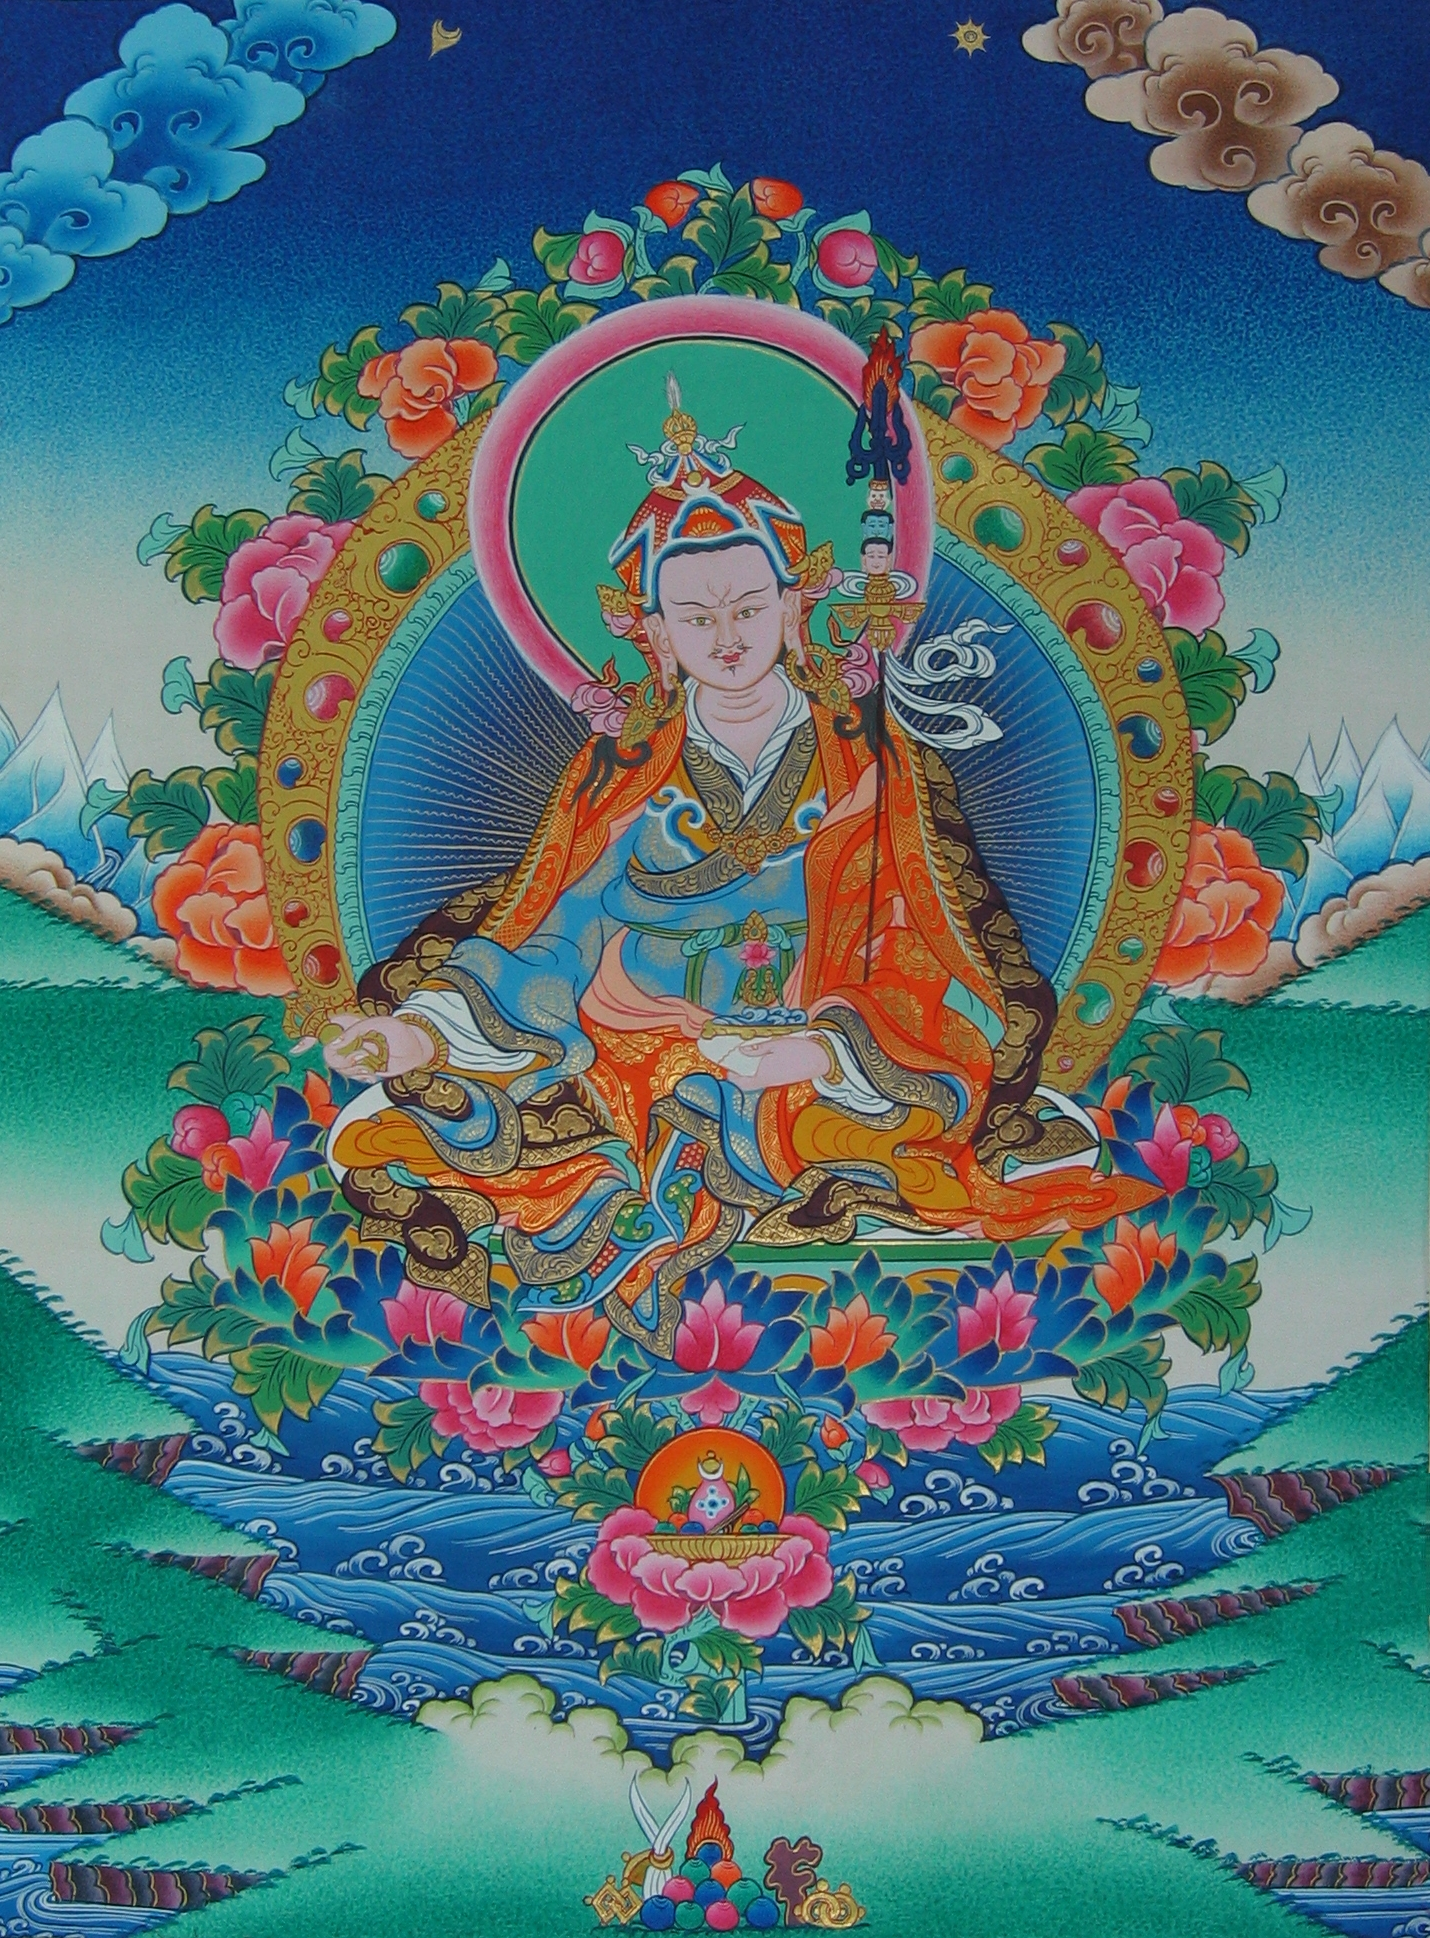
\includegraphics[scale=1]{guru_rinpoche.eps}}
\scaption{Le Pr�cieux Ma�tre (tib. Guru Rinpoche)}
\end{figure}
\vspace*{\stretch{1}}

\newpage

\titlesec{\Large Pri�re en sept lignes au Pr�cieux Ma�tre}
\addcontentsline{toc}{section}{\protect\numberline{}Pri�re en sept lignes}

\bigskip\bigskip

\begin{tabbing}
\stib{\swasti. \quad \myhung:} \quad
\=\stib{o rgyan yul gyi nub byang mtshams\notsheg:}\\
\>\lit{orgyen} \quad \ \ \=\lit{y�l} \=\lit{gyi} \=\lit{nub jang}
\=\lit{tsham}\\
\>\lex{O\d{d}\d{d}iy\a={a}na} \>\lex{pays} \>\lex{du}
\>\lex{nord-ouest} \>\lex{fronti�re}\\
\>\trans{Au nord-ouest du pays
  d'O\d{d}\d{d}iy\a={a}na,\sendnote{D'apr�s l'�rudition moderne,
  l'O\d{d}\d{d}iy\a={a}na serait une r�gion situ�e aux environs
  de la vall�e de Swat, au Pakistan. Consid�r�e aussi comme la patrie
  de Garab Dorje (Prahevajra), premier ma�tre humain de la
  Grande Perfection (tib. Dzogchen, skt. Mah\={a}sa\.{n}dhi) selon
  l'�cole des Anciens (tib. Nyingmapa). Au VII\ieme{} si�cle, le
  p�lerin chinois Xuanzang la traversa et d�crivit sa d�solation.}}\\
\>\stib{pa\V{d}{ma} ge sar sdong po la\notsheg:}\\
\>\lit{pema} \=\lit{gesar} \=\lit{dongpo} \=\lit{la}\\
\>\lex{lotus} \>\lex{pistil} \>\lex{tige} \>\lex{sur}\\
\>\trans{n� dans la corolle d'un lotus,}\\
\>\stib{ya mtshan mtshog gi dngos grub b-rnyis\notsheg:}\\
\>\lit{yatshen} \ \=\lit{chog} \quad \=\lit{gi} \=\lit{ng�drub} \quad
\quad \=\lit{nye}\\
\>\lex{merveilleux} \>\lex{supr�mes} \>\lex{de} \>\lex{accomplissements}
\>\lex{dot�}\\
\>\trans{dot� des r�alisations les plus merveilleuses,}
\end{tabbing}

\newpage

\begin{tabbing}
\=\stib{pa\V{d}{ma} 'byung gnas zhes su grags\notsheg:}\\
\>\lit{pema} \=\lit{jungne} \=\lit{shesu} \ \=\lit{drag}\\
\>\lex{lotus} \>\lex{n�} \>\lex{renomm�} \>\lex{comme}\\
\>\trans{vous �tes connu comme
  �~Celui-N�-du-Lotus~�\sendnote{tib. Guru Rinpoche,
    skt. Padmak\a={a}ra. Rigoureusement, Padmasambhava est le nom de
    l'un des huit aspects de Guru Rinpoche: l'�rudit, symbolisant la
    ma�trise de la philosophie. Il est ici repr�sent� sous sa forme la
    plus commune: si�giant sur un disque lunaire pos� sur un disque
    solaire dans la corolle d'un lotus; le regard si per�ant qu'il en
    �mane un sentiment de menace, mais sans courroux; il porte huits
    robes, symbolisant toutes les classes d'enseignements dont la
    Grande Perfection (tib. Dzogchen, skt. Mah\={a}sa\.{n}dhi) est le
    parach�vement; il tient dans sa main droite un \emph{vajra}
    (tib. \emph{dorje}), symbole d'infrangibilit� et des moyens
    salvifiques habiles; il tient de sa main gauche, pos�e dans le
    giron, une calotte cr�nienne emplie d'ambroisie, en guise
    d'aigui�re --- signe qu'il a vaincu la mort. Dans le creux du bras
    gauche il enserre un long trident en feu (symbolisant une arme
    contre les trois poisons: ignorance, d�sir et haine; la flamme
    d�notant la compassion active), orn� de trois t�tes coup�es (l'une
    fra�chement, l'autre cadav�rique, la derni�re est un cr�ne),
    symboles du triomphe total sur l'ego; il porte une coiffe en forme
    de lotus � cinq p�tales, symbolisant la famille � laquelle il
    appartient (cf. note 5), brod�e d'un croissant de lune et d'un
    soleil et surmont�e d'une plume de vautour, symbole de la Grande
    Perfection, ench�ss�e sur une pointe de \emph{vajra}. �tant un
    personnage historique (bien que les preuves soient rares), et bien
    que sublim� ici, sa peau est couleur chair.}}\\
\>\stib{'khor du mkha' 'gro mang ngos bskor\notsheg:}\\
\>\lit{khor du} \=\lit{khandro} \=\lit{mangp�} \=\lit{kor}\\
\>\lex{entourage} \>\lex{\emph{\d{d}\a={a}kin\a={\i}}}
\>\lex{nombreuses} \>\lex{entour�}\\
\>\trans{entour� de nombreuses
\emph{\d{d}\a={a}kin\a={\i}}.\sendnote{Les
  \emph{\d{d}\a={a}kin\a={\i}} sont des �tres spirituels f�minins.
  Il y en a deux sortes: les \emph{\d{d}\a={a}kin\a={\i}} de sagesse et les
  \emph{\d{d}\a={a}kin\a={\i}} mondaines. Ici il s'agit des premi�res,
  qui apparaissent dans le ciel et sont la manifestation visuelle de
  la vacuit� sous des formes particuli�rement nombreuses, c'est-�-dire
  qu'elles personnifient la r�alit� manifeste
  (\emph{sa\d{m}bhogak\a={a}ya}) en m�rissement, l'aboutissement
  �tant la reconnaissance de la r�alit� absolue
  (\emph{dharmak\a={a}ya}). En ce sens, elles sont souvent des
  messag�res, des interm�diaires ou des disciples d�vou�es � certaines
  d�it�s masculines (cette dualit� peut servir de base aux
  \emph{tantra} (skt.) d'union sexuelle et � l'iconographie des
  par�dres en union avec la d�it� masculine
  principale --- tib. \emph{yabyum}). Dans la perspective de la Grande
  Perfection (tib. Dzogchen, skt. Mah\={a}sa\.{n}dhi), en fixant le
  ciel d�gag�, elles
  apparaissent spontan�ment sous la forme de sph�res armillaires
  quinticolores (tib. \emph{thigle}, skt. \emph{bindu}) --- qui ne sont
  pas sans rappeler leurs bijoux �clatants --- et sont le signe du
  d�veloppement des visions extraordinaires.}}\\
\>\stib{khyed kyi rjes su bdga bsgrub kyis\notsheg:}\\
\>\lit{khye}-\=\lit{kyi} \=\lit{jesu} \=\lit{dag} \=\lit{drub}
\=\lit{kyi}\\
\>\lex{�} \>\lex{votre} \>\lex{suite} \>\lex{je} \>\lex{r�alise}
\>\lex{afin que}\\
\>\trans{Je suis celui qui suit vos pas,}\\
\>\stib{byin gyis b-rlab phyir gshegs su sol\notsheg:}\\
\>\lit{jin} \quad\qquad \=\lit{gyi lab} \=\lit{chir}
\=\lit{sheg su s�l}\\
\>\lex{b�n�diction} \>\lex{accordez} \>\lex{pour}
\>\lex{venez s'il vous pla�t}\\
\>\trans{je vous prie d'approcher et de me b�nir!}
\end{tabbing}

\bigskip

\titlesubsec{Formule}

\begin{tabbing}
\=\stib{gu ru pa\V{d}{ma} si\V{di}{dh} \myhung:}\\
\>\lit{guru} \=\lit{pema} \ \=\lit{siddhi} \quad \=\lit{hung}\\
\>\sans{guru} \>\sans{padma} \>\sans{siddhi}
\>\sans{h\a={u}\d{m}} \quad \textsf{[sanscrit]}\\
\>\lex{ma�tre} \>\lex{lotus} \>\lex{r�alisations}
\>\lex{syllabe-du-c{\oe}ur}\sendnote{\sans{h\a={u}\d{m}} est la syllabe
  associ�e � la roue du c{\oe}ur, donc � la r�alit� absolue
  (\emph{dharmak\a={a}ya}), et invoquant l'actualisation de l'union de
  l'aspect infrangible de l'esprit (sa nature �tant le vide
  d'existence intrins�que) et son aspect cognitif, ou clart�.}\\
\>\trans{R�alisations du Ma�tre du Lotus, soyez!...}
\end{tabbing}

\rep{� r�citer autant de fois que possible.}

\cleardoublepage
\
%%-*-latex-*-

\vspace*{\stretch{1}}
\begin{figure}[H]
\centering
\fbox{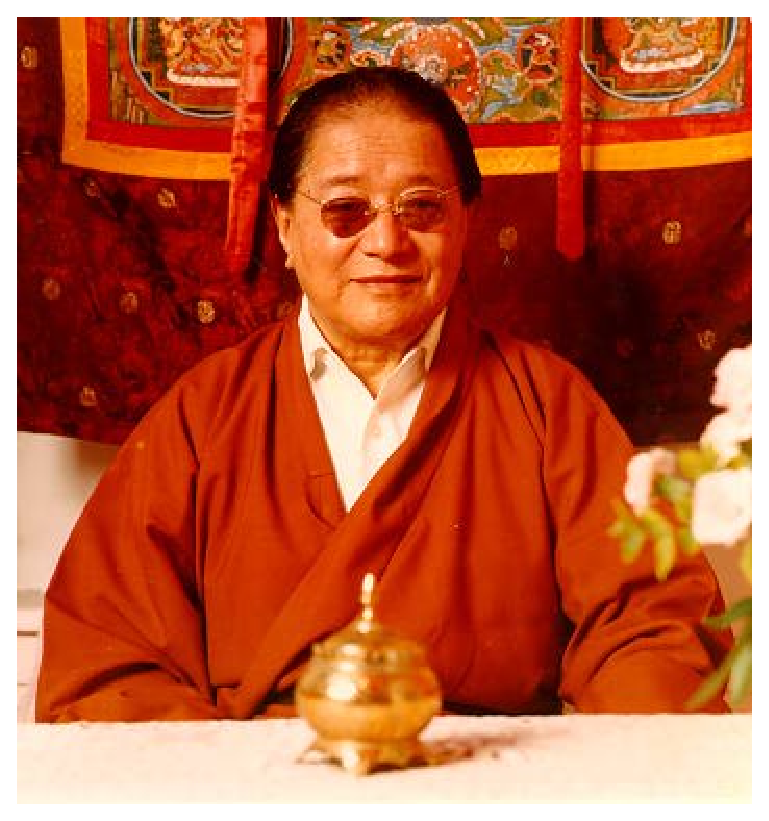
\includegraphics[scale=1]{dudjom.eps}}
\scaption{D�djom Rinpoche (1904-1987)}
\end{figure}
\vspace*{\stretch{1}}

\newpage

\titlesec{Appel au ma�tre qui est au loin\\
(chant de l'�tat naturel)}
\addcontentsline{toc}{section}{\protect\numberline{}Appel au ma�tre}

\bigskip\bigskip

\noindent{\large Tr�sor r�v�l� � Jigdrel Yeshe Dorje (alias D�djom
  Rinpoche).}

\bigskip\bigskip\bigskip


\titlesubsec{La r�alit� absolue} \hrulefill

\begin{tabbing}
\=\stib{\swasti..ngo bo gdod nas mi 'gyur spros bral gyi gshis lugs.}\\
\>\lit{ngowo} \=\lit{d�ne} \quad\ \ \=\lit{migyur}
\=\lit{tr�}---------\=\lit{drel} \=\lit{gyi} \=\lit{shilug}\\
\>\lex{essence} \>\lex{primordiale} \>\lex{immuable} \>\lex{�laboration}
\>\lex{libre} \>\lex{de} \>\lex{nature}\\
\>\trans{La nature fonci�re est � la fois puret� (sans �laborations)
sans origine}\\
\>\stib{.ka dga gting gsal gzhon nu bum sku ru bzhugs pa.}\\
\>\lit{kadag} \=\lit{ting}---\=\lit{sel} \ \ \=\lit{sh�nnu}
\=\lit{bum}-\=\lit{ku} \ \ \=\lit{ru} \=\lit{shugpa}\\
\>\lex{pure} \>\lex{profonde} \>\lex{clart�} \>\lex{jouvence}
\>\lex{vase} \>\lex{corps} \>\lex{tel} \>\lex{demeure}\\
\>\trans{et clart� latente (telle une lampe brillant dans un vase clos);}\\
\>\stib{.chos sku'i bla ma ye shes rdo rje de mkhyen no.}\\
\>\lit{ch�-kui} \ \=\lit{lama} \=\lit{yeshe} \=\lit{dorje} \qquad
\=\lit{de} \ \=\lit{khyen-no}\\
\>\lex{\emph{dharmak\a={a}ya}} \>\lex{ma�tre} \>\lex{sagesse}
\>\lex{indestructible} \>\lex{vous} \>\lex{qui savez}\\
\>\trans{� sage Yeshe Dorje (skt. Ghanavajra), ma�tre de la
r�alit� absolue,}\\
\>\stib{.lta ba'i gding chen thob para byin gyis rang rlobs shig.}\\
\>\lit{ta-w�} \=\lit{ding}-----\=\lit{chen} \=\lit{thob-pra}
\=\lit{jin} \lit{gyi} \=\lit{rang-lob} \=\lit{shig}\\
\>\lex{de la vue} \>\lex{confiance} \>\lex{grande} \>\lex{atteindre}
\>\lex{b�n�diction} \>\lex{accordez-moi} \>\lex{faites}\\
\>\trans{b�nissez-moi afin que j'�prouve et scelle l'�tat naturel!}
\end{tabbing}

\newpage

\titlesubsec{La r�alit� manifeste} \hrulefill

\begin{tabbing}
\=\stib{.rang bzhin ma 'gags zung 'djug 'od gsal gyi tshom bu.}\\
\>\lit{rang}-\=\lit{shin} \=\lit{magag} \=\lit{zungjug} \=\lit{�sel}
\=\lit{gyi} \=\lit{tshombu}\\
\>\lex{propre} \>\lex{nature} \>\lex{incessante} \>\lex{union}
\>\lex{clart�} \>\lex{de} \>\lex{gerbes}\\
\>\trans{La clart� ins�parable de la vacuit� se d�ploie en gerbes}\\
\>\stib{.lhun grub nges pa lnga ldan rol pa ru bzhugs pa.}\\
\>\lit{lh�ndrub} \=\lit{nepa} \quad\ \ \=\lit{na} \=\lit{den}
\=\lit{r�lpa} \=\lit{ru} \=\lit{shug pa}\\
\>\lex{spontan�es} \>\lex{perfections} \>\lex{cinq} \>\lex{ayant}
\>\lex{jeu} \>\lex{tel} \>\lex{demeure}\\
\>\trans{en tant que le jeu spontan� des Cinq
Perfections;}\sendnote{Selon la Grande Perfection
  (tib. Dzogchen, skt. Mah\={a}sa\.{n}dhi): %\footnum{1}
  \begin{enumerate}
    \item l'esprit naturel (tib. \emph{rigpa}), correspondant au
      ma�tre;
    \item l'espace de la puret� primordiale (\emph{dharmadh\={a}tu}),
      correspondant au lieu de l'enseignement;
    \item la fertilit� de cet espace (\emph{dharmat\={a}}),
      correspondant � l'assembl�e des \emph{bodhisattva};
    \item la manifestation spontan�e des cinq sagesses, correspondant
      � l'enseignement;
    \item l'intemporalit� (ou �~temps de Samantabhadra~�),
      correspondant au moment propice.
  \end{enumerate}
  Les cinq sagesses repr�sentent l'essence des cinq familles,
  c'est-�-dire les aspects �veill�s des cinq passions de base qui
  sont:
  \begin{enumerate}
    \item la na�vet�
      (sagesse du \emph{dharmadh\={a}tu}, famille de la roue, qui
      symbolise l'enseignement du Bouddha historique
      (\emph{tath\={a}gata}), bouddha Vairocana de couleur blanche,
      qualit� d'omnipr�sence, agr�gat de la forme, �l�ment espace);
    \item l'irascibilit� (sagesse du miroir, famille du diamant
      (\emph{vajra}), bouddha Ak\d{s}obhya de couleur bleue, qualit�
      de la clart� immuable, agr�gat de la conscience, �l�ment eau,
      direction de l'est, l'hiver);
    \item l'orgueil (sagesse de l'�galit�, famille du joyau
      (\emph{ratna}), bouddha Ratnasambhava de couleur jaune, qualit�
      de la g�n�rosit�, agr�gat des sensations, �l�ment terre,
      direction du sud, l'automne);
    \item le d�sir (sagesse du discernement, famille du lotus
      (\emph{padma}), bouddha Amit\={a}bha de couleur rouge, qualit�
      de la compassion, agr�gat des perceptions, �l�ment feu,
      direction de l'ouest, le printemps);
    \item la jalousie
      (sagesse de l'accomplissement, famille de l'activit�
      (\emph{karma}), bouddha Amoghasiddhi de couleur verte, qualit�
      de l'action juste, agr�gat des formations volitives, �l�ment du
      vent, direction du nord, l'�t�).
   \end{enumerate}}\\
\>\stib{.longs sku'i bla ma bde tshen rdo rje de mkhyen no.}\\
\>\lit{long-kui} \ \=\lit{lama}
\=\lit{de}-----\=\lit{chen} \=\lit{dorje} \qquad \=\lit{de}
\ \ \=\lit{khyen-no}\\ \>\lex{\emph{sa\d{m}bhogak\a={a}ya}}
\>\lex{ma�tre} \>\lex{f�licit�} \>\lex{grande} \>\lex{indestructible}
\>\lex{vous} \>\lex{qui savez}\\ \>\trans{� sage Dechen Dorje
  (skt. Mah\a={a}sukhavajra), ma�tre de la r�alit�
  manifeste,}\\ \>\stib{.sgom pa'i rtsal tshen rdzogs para byin gyis
  rang rlobs shig.}\\ \>\lit{gomp�} \ \=\lit{tsel} \ \ \=\lit{chen}
\=\lit{dzogpra} \=\lit{jin} \lit{gyi} \=\lit{rang-lob}
\=\lit{shig}\\ \>\lex{m�ditation} \>\lex{habilet�} \>\lex{grande}
\>\lex{perfectionner} \>\lex{b�n�diction} \>\lex{accordez-moi}
\>\lex{faites}\\ \>\trans{b�nissez-moi afin que je parach�ve la
  m�ditation!}
\end{tabbing}

\newpage
\label{compassion}

\titlesubsec{La r�alit� dynamique} \hrulefill

\begin{tabbing}
\=\stib{.thugs rje phyogs lhung bral ba mtha' grol gyi ye shes.}\\
\>\lit{thugje} \ \=\lit{chog}---\=\lit{lhung} \=\lit{drelwa}
\=\lit{tha} \=\lit{dr�l} \=\lit{gyi} \=\lit{yeshe}\\
\>\lex{compassion} \>\lex{partialit�} \>\lex{tomber} \>\lex{sans}
\>\lex{limite} \>\lex{libre} \>\lex{de} \>\lex{sagesse}\\
\>\trans{La compassion est sagesse illimit�e et impartiale,}\\
\>\stib{.kun khyab rig stong rjen pa'i ngo bo ru bzhugs pa.}\\
\>\lit{k�nkhyab} \ \=\lit{rig}---------\=\lit{tong} \=\lit{jenp�}
\=\lit{ngowo} \=\lit{ru} \ \=\lit{shug pa}\\
\>\lex{omnip�n�trante} \>\lex{conscience} \>\lex{vacuit�} \>\lex{nue}
\>\lex{essence} \>\lex{telle} \>\lex{demeure}\\
\>\trans{omnipr�sente car coessentielle � la nature fonci�re nue et
claire;}\\
\>\stib{.sprul sku'i bla ma 'gro 'dul gling pa de mkhyen no.}\\
\>\lit{tr�lkui} \ \ \=\lit{lama} \=\lit{drod�l} \=\lit{lingpa}
\=\lit{de} \ \=\lit{khyen-no}\\
\>\lex{\emph{nirm\a={a}\d{n}ak\a={a}ya}} \>\lex{ma�tre} \>\lex{Drod�l}
\>\lex{Lingpa} \>\lex{vous} \>\lex{qui savez}\\
\>\trans{� sage Drod�l Lingpa, ma�tre de la r�alit� dynamique,}\\
\>\stib{.spyod pa'i bogs tshen 'byongs para gyis rang rlobs shig.}\\
\>\lit{ch�}--\=\lit{p�} \=\lit{bog}---\=\lit{chen} \=\lit{jongpra}
\=\lit{jin} \lit{gyi} \=\lit{rang-lob} \=\lit{shig}\\
\>\lex{action} \>\lex{de} \>\lex{progr�s} \>\lex{grand}
\>\lex{accomplir} \>\lex{b�n�diction}
\>\lex{accordez-moi} \>\lex{faites}\\
\>\trans{b�nissez-moi afin que j'agisse habilement pour le bien
d'autrui!}
\end{tabbing}

\newpage

\titlesubsec{Conscience de soi et des objets}\hrulefill

\begin{tabbing}
\=\stib{.rang rig gdod ma'i gzhi la 'pho 'gyur ni mi 'dug.}\\
\>\lit{rang}-\=\lit{rig} \qquad\ \  \=\lit{d�m�} \quad\
\=\lit{shi}-\=\lit{la} \=\lit{pho}------\=\lit{gyur}
\=\lit{ni} \lit{midug}\\
\>\lex{de soi} \>\lex{conscience} \>\lex{primordiale}
\>\lex{base} \>\lex{est} \>\lex{bouge (ni)} \>\lex{change}
\>\lex{ne}\\
\>\trans{La conscience de soi\sendnote{La connaissance imm�diate
  et intuitive que la conscience a de ses propres modes,
  concomitamment � la perception de l'objet, est nomm�e
  \emph{svasamved\={a}na} en sanscrit. L'image traditionnelle
  est celle de la perception d'objets par la vue: cette conscience des
  formes est concomitante � la pr�sence de lumi�re, sans n�cessiter
  l'existence d'une autre lumi�re pour voir cette lumi�re ni une
  inf�rence logique pour conclure qu'il y a de la lumi�re. Ce vers et
  le suivant, en identifiant cette conscience r�flexive � la base
  primordiale qui est vide d'existence intrins�que, constitue une
  r�futation par l'�cole philosophique M\={a}dhyamika de
  la vue de l'Id�alisme bouddhique (\emph{cittam\={a}tra}) tardif
  qui tend � singuli�rement exalter cette conscience et donc � la
  r�ifier implicitement. Les perceptions varient (cf. vers suivant)
  mais cette conscience r�flexive est immuable \emph{car}
  intrins�quement vide (et pas seulement priv�e des objets per�us).}
  est immuable, n'�tant autre que la base primordiale;}\\
\>\stib{.gang shar chos sku'i rtsal la bzang ngan ni mi gda'.}\\
\>\lit{gang}--\=\lit{shar} \ \ \=\lit{ch�-kui}
\=\lit{tsel}------\=\lit{la} \=\lit{zang}-\=\lit{ngeng}
\=\lit{ni} \=\lit{mida}\\
\>\lex{quoi qui} \>\lex{appara�t} \>\lex{\emph{dharmak\a={a}ya}}
\>\lex{expression} \>\lex{est} \>\lex{bon (ni)} \>\lex{mauvais}
\>\lex{ni} \>\lex{n'est}\\
\>\trans{les ph�nom�nes sont efflorescence de la r�alit� absolue,
ni bons ni mauvais.}
\end{tabbing}

\titlesubsec{Le ma�tre} \hrulefill

\begin{tabbing}
\=\stib{.da lta'i shes pa sangs rgyas mngon sum du 'dug pas.}\\
\>\lit{da-t�} \quad \=\lit{shepa} \quad \=\lit{sangye} \=\lit{ng�nsum}
\=\lit{du} \ \=\lit{dug}-\=\lit{pe}\\
\>\lex{du pr�sent} \>\lex{conscience} \>\lex{Bouddha} \>\lex{r�alit�}
\>\lex{dans} \>\lex{est} \>\lex{comme}\\
\>\trans{Puisque l'�veil ne s'actualise que dans la conscience du pr�sent,}\\
\>\stib{.gu yangs blo bde'i bla ma snying dbus nas rnyed byung.}\\
\>\lit{gu}--\=\lit{yang} \qquad \ \ \=\lit{lodei} \=\lit{lama}
\=\lit{nying}-\=\lit{�} \quad \ \ \=\lit{ne} \ \=\lit{nye jung}\\
\>\lex{libre} \>\lex{compl�tement} \>\lex{serein} \>\lex{ma�tre}
\>\lex{c{\oe}ur} \>\lex{milieu} \>\lex{dans} \>\lex{est r�v�l�}\\
\>\trans{le ma�tre, totalement libre et serein, est r�v�l� dans le c{\oe}ur}\\
\>\stib{.gnyug ma'i sems 'di bla ma'i rang bzhin du rtogs tshe.}\\
\>\lit{nyugm�} \=\lit{sem} \=\lit{di} \=\lit{lam�} \=\lit{rang}-\=\lit{shin}
\=\lit{du} \quad \ \=\lit{tog} \ \=\lit{tshe}\\
\>\lex{inn�} \>\lex{esprit} \>\lex{cet} \>\lex{du lama}
\>\lex{m�me} \>\lex{nature} \>\lex{comme} \>\lex{r�alis�} \lex{quand}\\
\>\trans{quand on r�alise que cet esprit inn�\sendnote{La roue
    du c{\oe}ur est le si�ge de l'esprit inn�.} est la nature m�me du
  ma�tre,}\\
\>\stib{.'dzin zhen gsol 'debs bcos ma'i sdug yus ni ma dgos.}\\
\>\lit{dzinshen} \=\lit{s�ldeb} \=\lit{ch�m�}
\=\lit{dug-y�} \=\lit{ni} \lit{mag�}\\
\>\lex{tenaces} \>\lex{pri�res} \>\lex{factices} \>\lex{plaintes}
\>\lex{inutile}\\
\>\trans{et plus n'est besoin alors de pri�res tenaces ni de plaintes
factices.}
\end{tabbing}

\newpage

\titlesubsec{Le disciple (vue, m�ditation et activit�)}\hrulefill

\begin{tabbing}
\=\stib{.ma bcos rig pa rang bab kha yan du klod pas.}\\
\>\lit{ma-ch�} \quad \=\lit{rigpa} \qquad\quad \=\lit{rang}-\=\lit{bab}
\=\lit{khayen} \=\lit{du l� pe}\\
\>\lex{sans entraves} \>\lex{conscience claire} \>\lex{propre} \>\lex{cours}
\>\lex{libre} \>\lex{se laisser aller}\\
\>\trans{Suivant librement le cours propre de la conscience claire
inobstru�e,}\\
\>\stib{.gtad med gang shar rang grol byin rlabs de thob byung.}\\
\>\lit{te-me} \quad \=\lit{gang}-\=\lit{shar} \
\=\lit{rang-dr�l} \=\lit{jinlab} \ \=\lit{de thob jung}\\
\>\lex{ne pas saisir} \>\lex{quoi qui} \>\lex{surgisse}
\>\lex{auto-lib�ration} \>\lex{b�n�diction} \>\lex{sont obtenus}\\
\>\trans{sans saisir, les ph�nom�nes jaillisent alors naturellement
libres.}\\
\>\stib{.byas pa'i chos kyis sangs rgyas 'grub dus ni mi gda'.}\\
\>\lit{jep�} \=\lit{ch�} \quad \=\lit{kyi} \=\lit{sangye} \=\lit{drub}
\=\lit{d�} \qquad \lit{ni} \=\lit{mida}\\
\>\lex{factice} \>\lex{pratique} \>\lex{par} \>\lex{l'�veil}
\>\lex{atteint} \>\lex{moment} \>\lex{a aucun}\\
\>\trans{Aucune fabrication ne menant � l'�veil,}\\
\>\stib{.yid dpyod blos byas sgom 'di bslu byed kyi dgra red.}\\
\>\lit{yi}------\=\lit{ch�} \ \ \=\lit{l�}------\=\lit{je} \quad \ \
\=\lit{gom} \quad \ \ \=\lit{di} \ \ \=\lit{luje} \ \=\lit{kyi}
\=\lit{dra} \ \=\lit{re}\\
\>\lex{mentale} \>\lex{analyse} \>\lex{intellect} \>\lex{produit}
\>\lex{m�ditation} \>\lex{cette} \>\lex{tromper} \>\lex{de}
\>\lex{ennemi} \>\lex{est}\\
\>\trans{la m�ditation cr��e par l'activit� mentale est l'ennemi
trompeur.}\\
\>\stib{.da ni 'dzin stangs zhig pa'i mto med kyi smyon pa.}\\
\>\lit{da}---------\=\lit{ni} \=\lit{dzintang}
\quad \=\lit{shig}-\=\lit{p�} \quad \ \=\lit{dome} \=\lit{kyi}
\=\lit{ny�npa}\\
\>\lex{maintenant} \>\lex{l�} \>\lex{conceptualisation}
\>\lex{laisser} \>\lex{tomber} \>\lex{abandon} \>\lex{de}
\>\lex{un fou}\\
\>\trans{Ainsi, tel un fou, j'abandonne ici et maintenant les concepts}\\
\=\stib{.byung rgyal gcer nyal ngang la mi tshe 'di skyel gtong.}\\
\>\lit{junggyel} \=\lit{cher} \=\lit{nyel} \
\=\lit{ngang-la} \=\lit{mitshe} \ \=\lit{di} \ \
\=\lit{kyeltong}\\
\>\lex{sans inhibitions} \>\lex{nue} \>\lex{qui�tude}
\>\lex{�tat-dans} \>\lex{vie humaine} \>\lex{cette} \>\lex{se
  d�roule}\\
\>\trans{pour vivre une qui�tude simple, sans espoir ni crainte.}
\end{tabbing}

\newpage

\titlesubsec{La voie de D�djom}\hrulefill

\begin{tabbing}
\=\stib{.gang ltar byas kyang dga'o rdzogs chen gyi rnal 'byor.}\\
\>\lit{gang-tar} \=\lit{je} \=\lit{kyang} \=\lit{gao} \
\=\lit{dzog}-----\=\lit{chen} \=\lit{gyi} \=\lit{neljor}\\
\>\lex{quoi qui (est)} \>\lex{fait} \>\lex{aussi} \>\lex{joyeux}
\>\lex{perfection} \>\lex{grande} \>\lex{de} \>\lex{pratiquant}\\
\>\trans{Joyeux quoi qu'il fasse, le pratiquant de la Grande
Perfection}\\
\>\stib{.su dang 'grogs kyang skyid do pad 'byung gi bu rgyud.}\\
\>\lit{su-dang} \=\lit{drog} \quad \=\lit{kyang} \=\lit{kyido}
\=\lit{pejung} \quad \=\lit{gi} \=\lit{bu} \=\lit{gy�}\\
\>\lex{dans chaque} \>\lex{compagnie} \>\lex{aussi} \>\lex{heureux}
\>\lex{N�-du-Lotus}\sendnote{Ce chant est un tr�sor spirituel de Guru
  Rinpoche (skt. Padmak\={a}ra) r�v�l� � D�djom Rinpoche. Ici,
  Guru Rinpoche fait r�f�rence � D�djom Rinpoche et � ses disciples,
  qu'il consid�re comme ses propres fils spirituels.} \>\lex{de}
\>\lex{fils} \>\lex{lign�e}\\
\>\trans{est heureux en toute compagnie et est le digne fils spirituel
de D�djom,}\\
\>\stib{.mgon la 'gran zla med do gter chen gyi bla ma.}\\
\>\lit{g�nla} \quad \=\lit{drenda} \=\lit{me do}
\=\lit{ter}---------\=\lit{chen} \=\lit{gyi} \=\lit{lama}\\
\>\lex{protecteur} \>\lex{rival} \>\lex{sans}
\>\lex{tib. \emph{tert�n}} \>\lex{grand} \>\lex{de} \>\lex{ma�tre}\\
\>\trans{le protecteur nonpareil (des enseignements), l'h�ritier de
mes tr�sors}\\
\>\stib{.chos la do zla med do mkha' 'gro yi snying thig.}\\
\>\lit{ch�} \lit{la} \quad \ \=\lit{doda} \qquad \=\lit{me} \lit{do}
 \=\lit{khandro} \=\lit{yi} \=\lit{nying}-\=\lit{thig}\\
\>\lex{\emph{dharma}} \>\lex{comparaison} \>\lex{au-del�}
\>\lex{\emph{\d{d}\a={a}kin\a={\i}}} \>\lex{de}
\>\lex{c{\oe}ur} \>\lex{essence}\\
\>\trans{et dont la voie incomparable m�ne � l'essence du c{\oe}ur des
  \emph{\d{d}\a={a}kin\a={\i}}.}\\
\>\stib{.rmongs chen snying gi mun pa rang mal du sangs nas.}\\
\>\lit{mong}---\=\lit{chen} \=\lit{nying} \=\lit{gi} \=\lit{m�npa}
\=\lit{rang}-\=\lit{mel} \=\lit{du} \=\lit{sang} \=\lit{ne}\\
\>\lex{ignorance} \>\lex{grande} \>\lex{c{\oe}ur} \>\lex{du}
\>\lex{t�n�bres} \>\lex{propre} \>\lex{lieu} \>\lex{en}
\>\lex{purifi�} \>\lex{ayant}\\
\>\trans{Les t�n�bres du c{\oe}ur seront dissip�es sur place}\\
\stib{.'od gsal nyi ma 'grib med khor yug tu 'char ba'i.}\\
\>\lit{�sel} \=\lit{nyima} \=\lit{drib-me} \=\lit{khoryug} \lit{tu}
\=\lit{charw�}\\
\>\lex{clart�} \>\lex{soleil} \>\lex{sans voiles} \>\lex{contin�ment}
\>\lex{se lever}\\
\>\trans{par la clart� continue du soleil levant dans le ciel sans
nuages.}
\end{tabbing}

\newpage

\titlesubsec{La d�votion au ma�tre} \hrulefill

\begin{tabbing}
\=\stib{.skal bzang 'di ko pha gcig bla ma yi sku drin.}\\
\>\lit{kelzang} \ \ \=\lit{di} \lit{ko} \=\lit{pha}-\=\lit{chig}
\=\lit{lama} \=\lit{yi} \=\lit{kudrin}\\
\>\lex{bonne fortune} \>\lex{cette} \>\lex{p�re} \>\lex{unique}
\>\lex{ma�tre} \>\lex{de} \>\lex{bont�}\\
\>\trans{Cette bonne fortune est la bont� du ma�tre, mon unique
p�re.}\\
\>\stib{.drin lan 'khor mtha' med do bla ma rang dran no.}\\
\>\lit{drinlen} \=\lit{khortha} \=\lit{me do} \quad \=\lit{lama}
\=\lit{rang} \quad \=\lit{dren-no} \textbf{[ter]}\\
\>\lex{bont�} \>\lex{rembourser} \>\lex{on ne peut}
\>\lex{ma�tre} \>\lex{seulement} \>\lex{(je) me souviens}\\
\>\trans{Ma�tre que l'on ne peut payer de retour, je n'ai que vous �
l'esprit!}
\end{tabbing}

\vspace*{\stretch{1}}

\begin{figure}[H] \centering
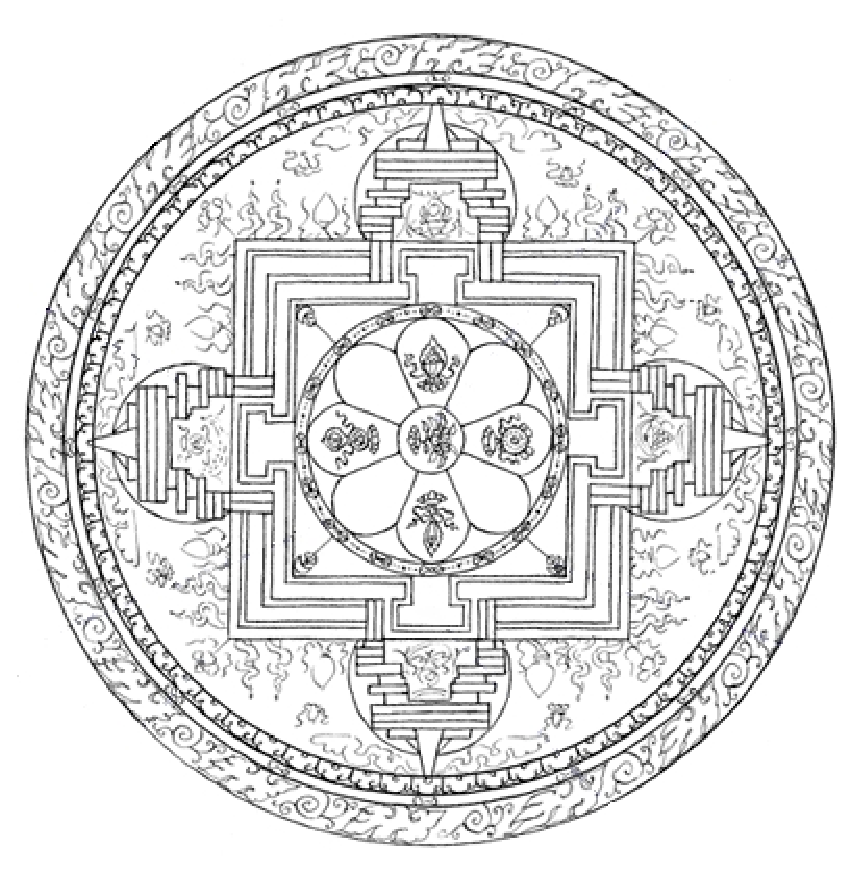
\includegraphics[scale=0.6]{mandala.eps}
\scaption{\emph{ma\d{n}\d{d}ala}}
\end{figure}

\vspace*{\stretch{1}}

%%-*-latex-*-

\vspace*{\stretch{1}}

\begin{figure}[!h]
\centering
\fbox{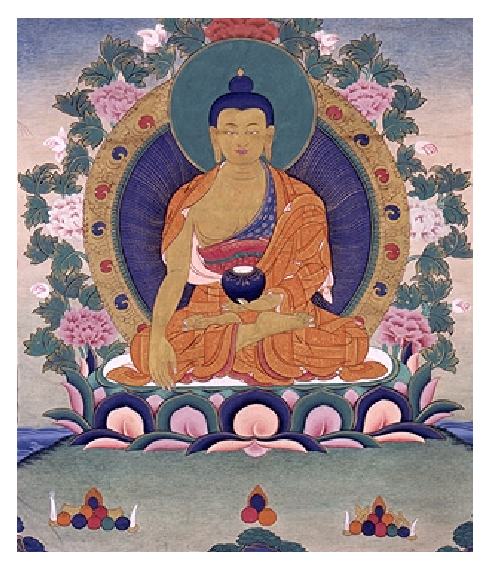
\includegraphics[scale=1.2]{sakyamuni.eps}}
\scaption{Le Bouddha}
\end{figure}

\vspace*{\stretch{1}}

\newpage

\titlesec{Les quatre pens�es qui d�tournent du cycle}
\addcontentsline{toc}{section}{\protect\numberline{}Les quatre pens�es}

\bigskip\bigskip

\begin{tabbing}
\=\stib{namo\notsheg:} \quad\
\=\stib{bslu med gtangyi mgonpo blama mkhyen\notsheg:}\\
\>\lit{namo} \>\lit{lume} \ \ \=\lit{ten}--------\=\lit{gyi}
\=\lit{g�npo} \ \=\lit{lama} \=\lit{khyen}\\
\>\lex{hommage} \>\lex{infaillible} \>\lex{constance} \>\lex{avec}
\>\lex{protecteur} \>\lex{ma�tre} \>\lex{qui sait}\\
\>\trans{Hommage au ma�tre patient et s�r, le protecteur, celui qui sait!}
\sendnote{Cette section est plac�e sous les auspices du Bouddha
  historique car elle est le point de d�part du voyage, tout comme le
  Bouddha a �t� le premier � montrer la voie. Celui-ci est repr�sent�
  ici assis dans la posture du lotus sur un disque lunaire reposant
  dans la corolle d'un lotus. Il est v�tu d'une robe monastique et
  coiff� d'un chignon. (Nul ne sait pourquoi, alors que le Bouddha se
  rasait les cheveux. Peut-�tre est-ce la protub�rance apicale
  cr�nienne, l'une des marques corporelles d'un �veill�, qui finit par
  �tre recouverte de cheveux par l'iconographie?) Il tient dans main
  gauche, pos�e sur son giron, un bol � offrande orn�; de la main
  droite il fait le le sceau (\emph{mudr\a={a}}) de la �~prise �
  t�moin de la terre~� (\emph{bh\a={u}mispar\a'{s}amudr\a={a}}), geste
  qu'il fit apr�s avoir atteint l'�veil complet, en r�ponse � une
  ultime tentative de Mar\={a}, le dieu en charge du cycle des
  renaissances (\emph{sa\d{m}s\={a}ra}), pour le faire
  douter de son accomplissement.}
\end{tabbing}
\hrulefill
\begin{tabbing}
\=\stib{dal 'byor 'di ni shin tu rnyed par dka'\notsheg:}\\
\>\lit{del}---\=\lit{jor} \quad \ \=\lit{di} \quad \=\lit{ni}
\=\lit{shintu} \qquad \quad\ \ \=\lit{nye}--\=\lit{par} \ \ \=\lit{ka}\\
\>\lex{libert�} \>\lex{dotation} \>\lex{cette} \>\lex{l�}
\>\lex{(est) extr�mement} \>\lex{�} \>\lex{obtenir} \>\lex{difficile}\\
\>\trans{Notre libert� pr�sente est extr�mement difficile � obtenir;}\\
\>\stib{skye tshad mi rtag 'chi ba'i chos can yin\notsheg:}\\
\>\lit{kye}-\=\lit{tshe} \qquad \ \ \=\lit{mitag} \qquad \=\lit{chiw�}
\=\lit{ch�}-\=\lit{chen} \=\lit{yin}\\
\>\lex{na�t} \>\lex{tout (ce qui)} \>\lex{impermanent} \>\lex{mort}
\>\lex{loi} \>\lex{ayant} \>\lex{est}\\
\>\trans{il est de la nature de ce qui na�t d'�tre impermanent et mortel;}\\
\>\stib{dge sdig las kyi rgyu 'bras bslu ba med\notsheg:}\\
\>\lit{ge}---\=\lit{dig} \=\lit{le}-----\=\lit{kyi}
\=\lit{gyu}-\=\lit{dre} \quad \=\lit{luwa} \=\lit{me}\\
\>\lex{vertu} \>\lex{vice} \>\lex{actes} \>\lex{des}
\>\lex{cause} \>\lex{r�sultat} \>\lex{(sont) inexorables}\\
\>\trans{l'encha�nement des actes, vertueux ou non, est inexorable;}\\
\>\stib{khams gsum 'khor ba sdug bsngal rgya s-tsho'i
  ngang\notsheg:}\\
\>\lit{kham}---\=\lit{sum} \=\lit{khorwa} \=\lit{dugnel}
\=\lit{gyats�} \=\lit{nang}\\
\>\lex{royaumes} \>\lex{trois} \>\lex{\emph{sa\d{m}s\a={a}ra}}
\>\lex{souffrance} \>\lex{oc�an} \>\lex{nature}\\
\>\trans{la nature de l'existence cyclique est oc�an de souffrances.}\\
\>\stib{dran nas bdag blo chos la 'gyur bar shog\notsheg:}\\
\>\lit{dren-ne} \=\lit{dag-lo} \ \=\lit{ch�} \=\lit{la} \qquad
\=\lit{gyurwar} \=\lit{shog}\\
\>\lex{me souvenir} \>\lex{mon esprit} \>\lex{voie} \>\lex{vers (la)}
\>\lex{se tourner} \>\lex{puisse}\\
\>\trans{M'en souvenant, puisse mon esprit se tourner vers la voie!}
\end{tabbing}

\rep{� r�citer trois fois les mains jointes en pri�re.}

%%-*-latex-*-

\vspace*{\stretch{1}}

\begin{figure}[H] \centering
\fbox{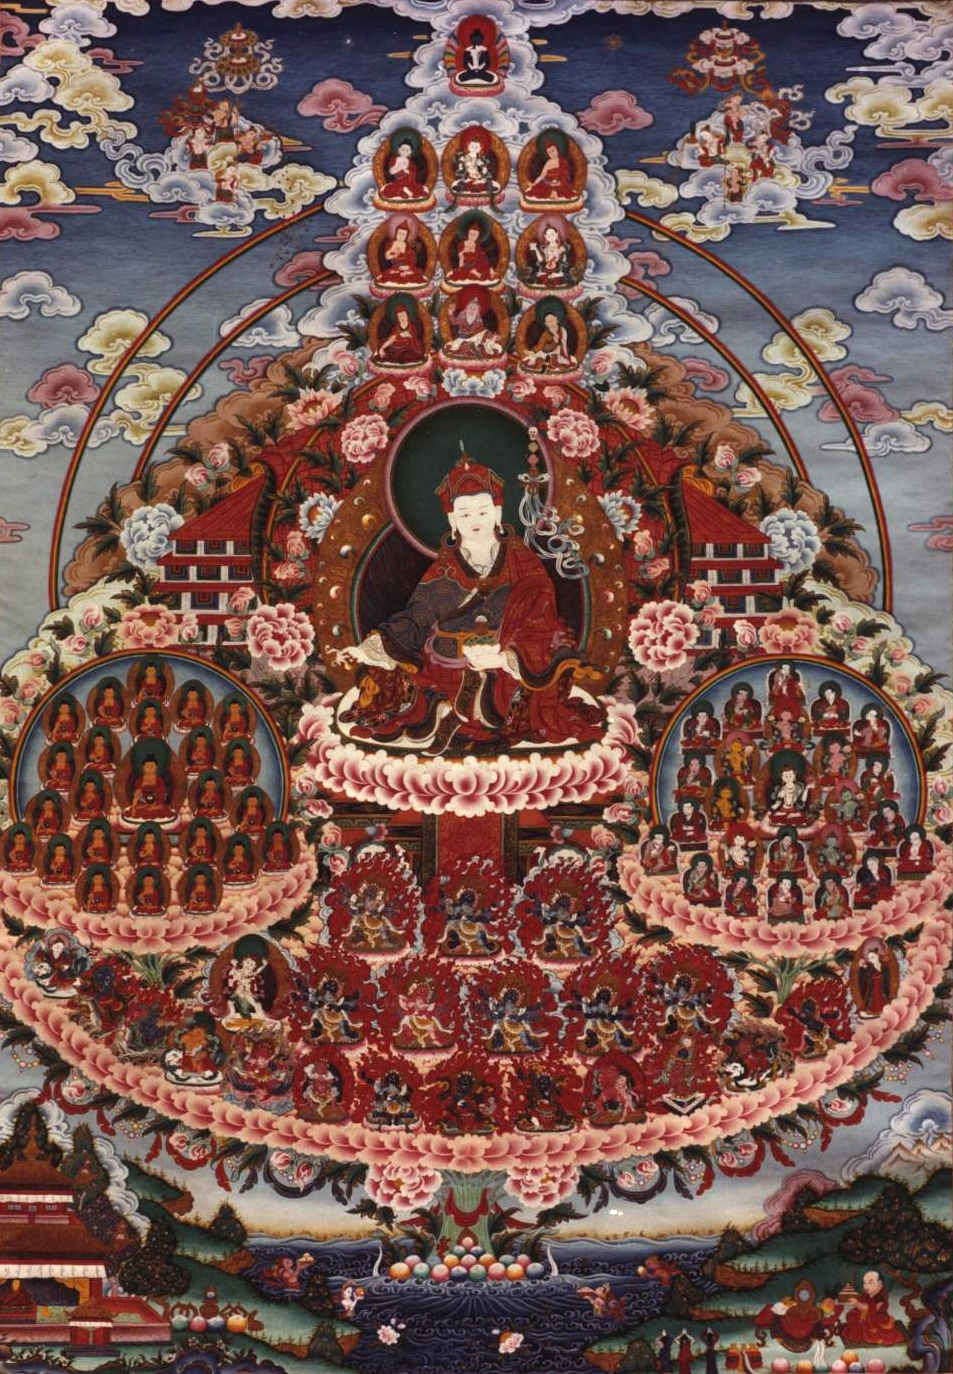
\includegraphics[scale=0.7]{refuge_tree.eps}}
\scaption{L'arbre de la lign�e Tersar}
\end{figure}

\vspace*{\stretch{1}}

\pagebreak

\titlesec{Refuge, aspiration d'�veil et offrande}
\addcontentsline{toc}{section}{\protect\numberline{}Refuge, aspiration
  d'�veil et offrande}

\bigskip\bigskip

\begin{tabbing}
\=\stib{'di bzung byang chub snying po ma thob bar\notsheg:}\\
\>\lit{di}--------------\=\lit{sung} \=\lit{jangchub} \=\lit{nyingpo}
\=\lit{ma}-\=\lit{thob} \ \=\lit{bra}\\
\>\lex{maintenant} \>\lex{depuis} \>\lex{�veil} \>\lex{c{\oe}ur}
\>\lex{pas} \>\lex{atteint} \>\lex{tant que}\\
\>\trans{D�sormais et jusqu'� ce que j'atteigne le c{\oe}ur de l'�veil,}\\
\>\stib{bla ma dkon mchog gsum la skyabs su mchi\notsheg:}\\
\=\lit{lama} \=\lit{k�nchog} \=\lit{sum} \=\lit{la} \=\lit{kyab su chi}\\
\>\lex{ma�tre} \>\lex{pr�cieux} \>\lex{trois} \>\lex{en}
\>\lex{je prends refuge}\\
\>\trans{je prends refuge dans le ma�tre et les Trois
Joyaux.}\sendnote{Les Trois Joyaux (\emph{triratna}) sont le
  Bouddha, la voie qu'il a montr�e (\emph{dharma}) et la
  communaut� (monastique et la�que r�unies, skt. \emph{sa\.{n}gha})
  qui la parcourt.}\\
\>\stib{da nas bzung ste 'khor ba ma stong bar\notsheg:}\\
\=\lit{da-ne}-----\=\lit{sung-te} \=\lit{khorwa} \quad \
\=\lit{ma}-\=\lit{tong} \=\lit{bra}\\
\>\lex{maintenant} \>\lex{depuis} \>\lex{\emph{sa\d{m}s\a={a}ra}}
\>\lex{non} \>\lex{vide} \>\lex{tant que}\\
\>\trans{D�sormais et tant que les mondes seront peupl�s,}\\
\>\stib{ma gyur sems can kun gyi phan bde bsgrub\notsheg:}\\
\>\lit{ma}---\=\lit{gyur} \quad \ \=\lit{semchen} \=\lit{k�n}-\=\lit{gyi}
\=\lit{phen}---\=\lit{de} \qquad \=\lit{drub}\\
\>\lex{m�re} \>\lex{(ayant) �t�} \>\lex{�tres} \>\lex{tous} \>\lex{de}
\>\lex{b�n�fice} \>\lex{bonheur} \>\lex{accomplir}\\
\>\trans{j'{\oe}uvrerai au bonheur des �tres, mes anciennes m�res.}
\end{tabbing}

\rep{� r�citer trois fois les mains jointes en pri�re (ou une fois en
  se prosternant).}

\begin{tabbing}
\=\stib{tshe rabs kun gyi lus dang longs spyod dpal\notsheg:}\\
\>\lit{tshe}-\=\lit{rab} \quad \ \ \=\lit{k�n}-\=\lit{gyi} \=\lit{l�}
\ \ \=\lit{dang} \=\lit{long} \=\lit{ch�} \=\lit{pel}\\
\>\lex{vies} \>\lex{succession} \>\lex{tous} \>\lex{de} \>\lex{corps}
\>\lex{et} \>\lex{joies} \>\lex{biens} \>\lex{honneurs}\\
\>\trans{Dans ma vie et les suivantes, corps, biens et honneurs,}\\
\>\stib{tshogs gnyis rdzogs phyir dkon mchog gsum la 'bul\notsheg:}\\
\>\lit{tshog}--------\=\lit{nyi} \=\lit{dzog} \quad \=\lit{chir}
\=\lit{k�nchog} \=\lit{sum} \=\lit{la} \=\lit{b�l}\\
\>\lex{accumulations} \>\lex{deux} \>\lex{completer} \>\lex{afin de}
\>\lex{joyaux} \>\lex{trois} \>\lex{aux} \>\lex{offrir}\\
\>\trans{je les offre aux Trois Joyaux afin d'accumuler m�rites et sagesse.}
\end{tabbing}

\rep{� r�citer trois fois en formant le sceau du \emph{ma\d{n}\d{d}ala} au
  niveau de la roue du c{\oe}ur (ou en faisant l'offrande rituelle).}

%%-*-latex-*-

\addcontentsline{toc}{section}{\protect\numberline{}Repentir et purification}

\vspace*{\stretch{1}}
\begin{figure}[H]
\centering
\fbox{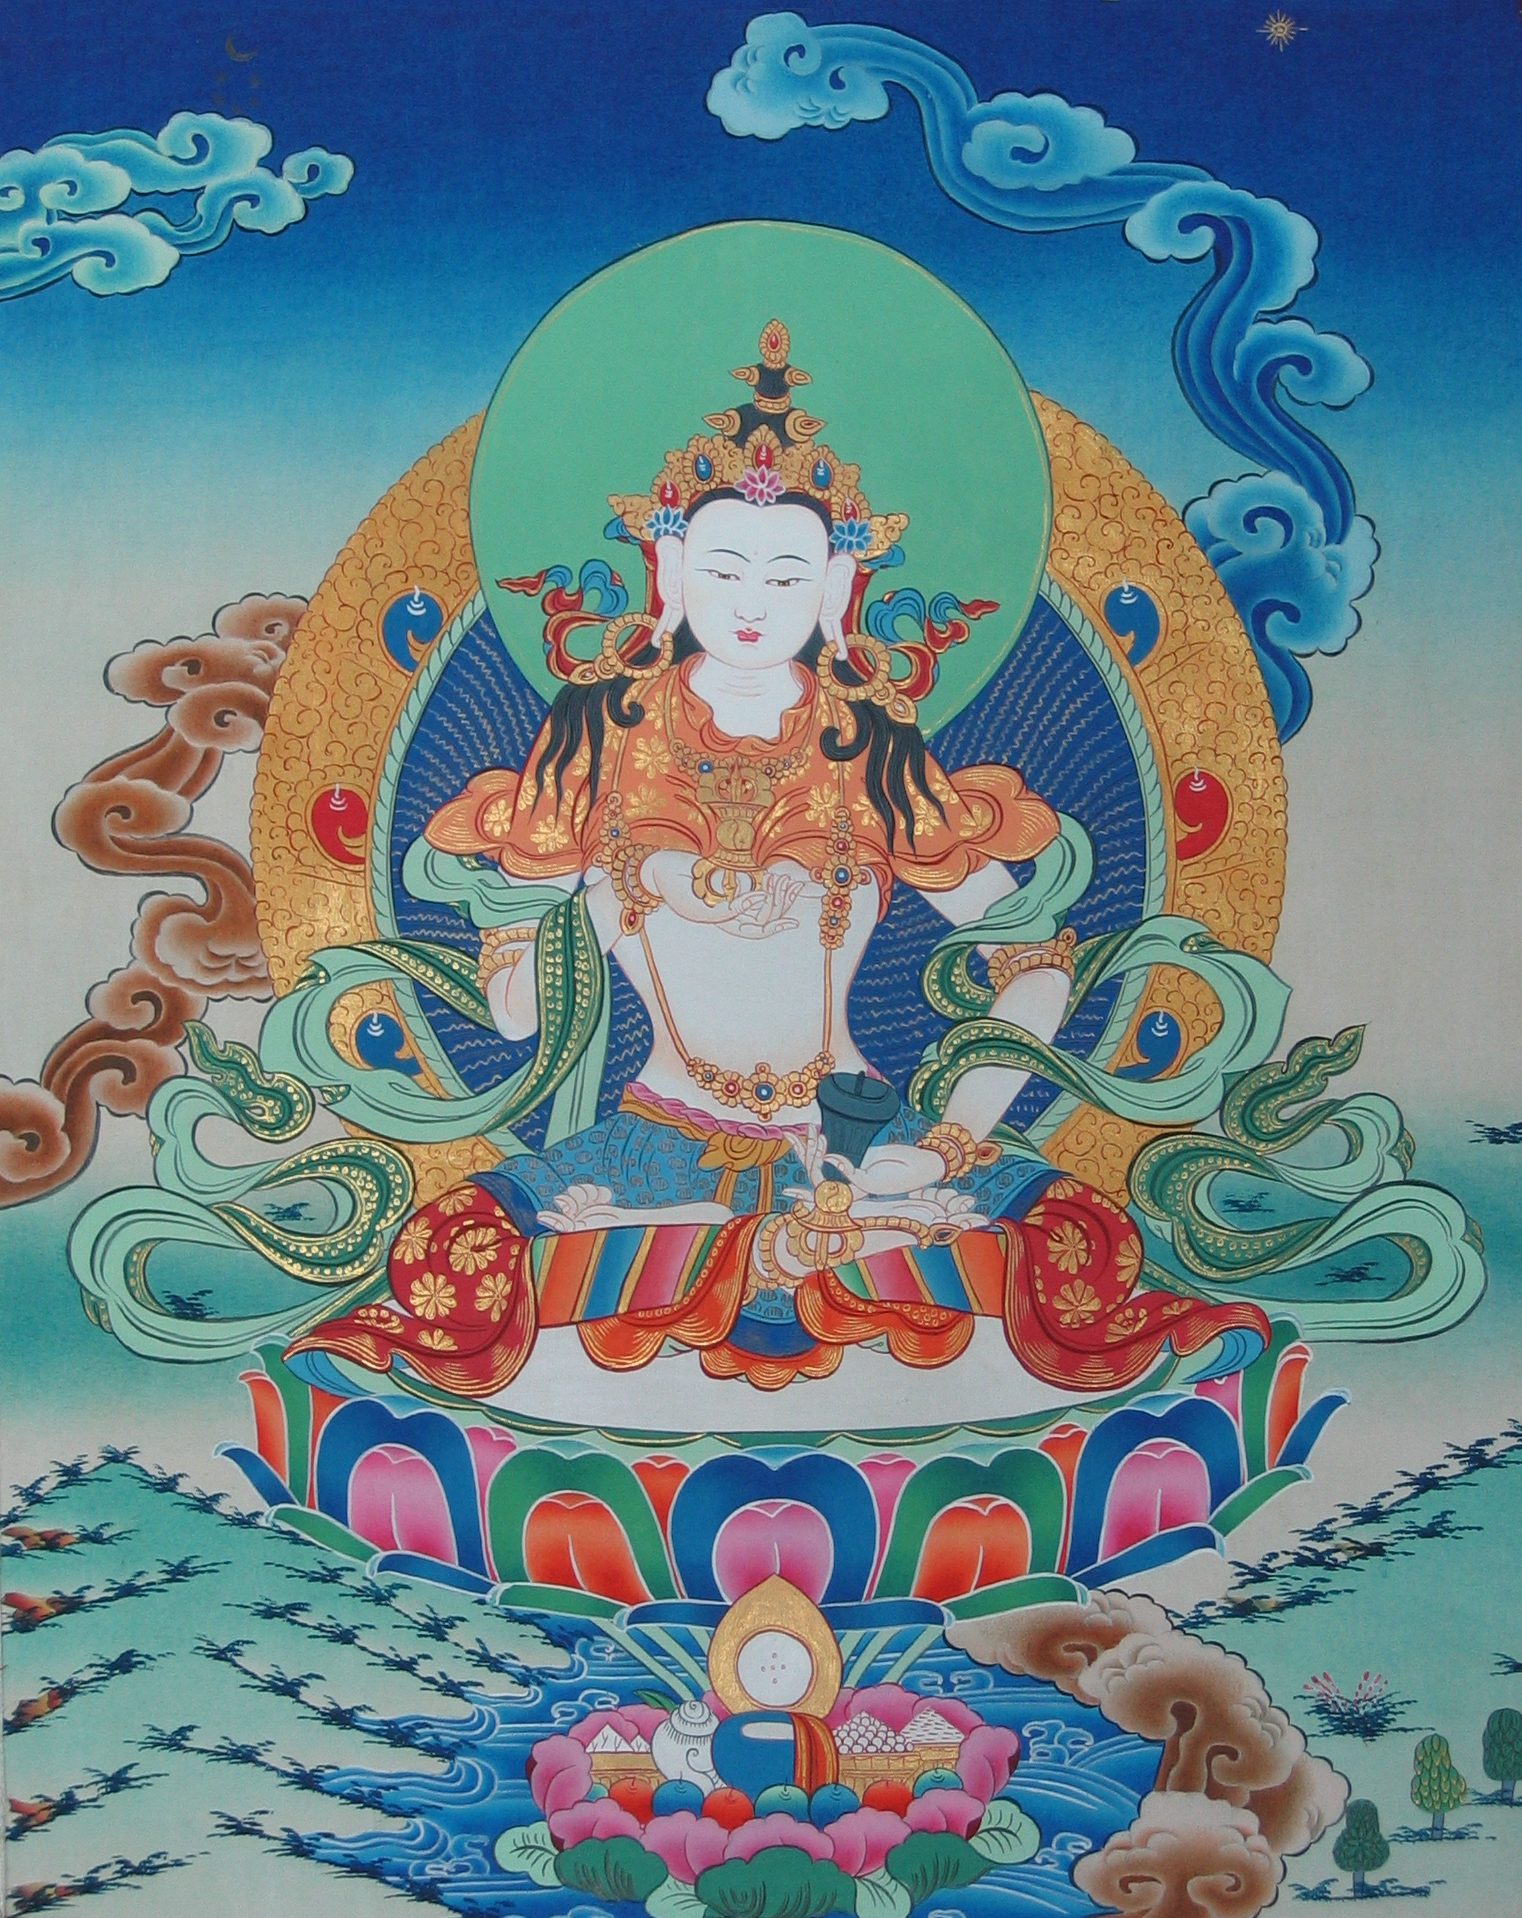
\includegraphics[scale=1]{vajrasattva.eps}}
\scaption{Vajrasattva (tib. Dorje Sempa)}
\end{figure}
\vspace*{\stretch{1}}

\newpage

\titlesec{Repentir et purification}

\bigskip\bigskip\bigskip\bigskip

\titlesubsec{Cr�ation}

\begin{tabbing}
\=\stib{spyi bor bla ma rdor sems dbyer med
  pa'i\notsheg:}\\ \>\lit{chiwor} \qquad \ \ \=\lit{lama}
\=\lit{dorsem} \quad\qquad \=\lit{yerme}---\=\lit{p�}\\ \>\lex{sommet
  du cr�ne} \>\lex{ma�tre} \>\lex{tib. \emph{\emph{Dor}je
    \emph{Sem}pa}} \>\lex{ins�parable} \>\lex{de}\\ \>\trans{Le
  ma�tre, ins�parable de Vajrasattva,\sendnote{La d�it� de support �
    la purification des fautes est nomm�e \emph{Dorje Sempa} en
    tib�tain. Il est l'�veill� manifestant la r�alit� absolue dans sa
    dimension de puret� sans origine (absence d'�laborations duelles,
    hors du temps). Sa couleur blanche brillante symbolise la
    personnification de tous les �veill�s, comme l'�veill� Vairocana
    (cf. famille de la roue, note 5) au centre du
    \emph{ma\d{n}\d{d}ala} des Cinq Familles, donc sa capacit� �
    absoudre toutes les sortes de fautes. (La lumi�res blanche
    contient potentiellement toutes les autres couleurs.) Vajrasattva
    �tant une �manation du Vainqueur Ak\d{s}obhya (cf. famille du
    diamant, note 5), cette pratique non seulement est un puissant
    moyen de purification de toutes les fautes mais en particulier un
    antidote � la haine, la col�re, l'aversion, l'irascibilit�
    etc. (L'ire est souvent consid�r�e comme la plus grande des fautes
    puisqu'elle obscurcit la compassion, vertu cardinale, ce qui n'est
    pas le cas de la luxure, par exemple.) Son expression et son
    environnement sont paisibles, induisant ainsi � la pratique les
    charact�res col�riques. Il tient, dans la main droite, � hauteur
    du plexus solaire (en fait, la roue du c{\oe}ur), un \emph{vajra}
    (tib. \emph{dorje}) d'or, symbole d'infrangibilit� et des moyens
    salvifiques habiles (\emph{up\a={a}ya}), c'est-�-dire de la
    compassion en action (cf. esprit d'�veil ou \emph{bodhicitta}
    relative) ---~relevant de la polarit� masculine. De la main
    gauche, il tient contre l'aine une clochette muette, symbole de
    \emph{praj�\a={a}}, l'exp�rience directe de la vacuit� des
    ph�nom�nes (cf. esprit d'�veil ou \emph{bodhicitta} absolue)
    ---~relevant de la polarit� f�minine. L'union de \emph{up\a={a}ya}
    et \emph{praj�\a={a}} est indispensable pour atteindre l'�veil
    pour soi et autrui. Vajrasattva est assis sur un disque lunaire
    pos� dans la corolle d'un lotus. La lune et le lotus, en s'�levant
    immacul�s, respectivement au-dessus des nuages et des eaux
    fangeuses, symbolisent la puret� inalt�rable de l'esprit, en
    d'autres termes, la vacuit� des �laborations mentales, et c'est
    ainsi que lune et lotus symbolisent
    \emph{praj�\a={a}}. Vajrasattva est coiff� d'une tiare, signe
    qu'il r�gne sur l'assembl�e (\emph{ma\d{n}\d{d}ala}) de toutes les
    d�it�s. Ses autres attributs, v�tements et bijoux, d�notent la
    r�alit� manifeste (\emph{sa\d{m}bhogak\a={a}ya}).}  s'assoie au
  sommet du cr�ne,}\\ \>\stib{sku las bdud rtsi'i rgyun babs sgrib
  sbyangs gyur\notsheg:}\\ \>\lit{ku}---\=\lit{le} \=\lit{d�tsi}
\=\lit{gy�n}-\=\lit{bab} \quad \=\lit{drib}
\qquad\qquad\ \ \=\lit{jang} \lit{gyur}\\ \>\lex{corps} \>\lex{du}
\>\lex{nectar} \>\lex{flot} \>\lex{descend} \>\lex{obscursissements}
\>\lex{purifiant}\\ \>\trans{de son corps coule un flot de nectar
  purifiant mes fautes.}
\end{tabbing}

\bigskip\bigskip

\titlesubsec{Formule aux cents syllabes}

\begin{tabbing}
\=\stib{\om\notsheg:} \quad
\=\stib{badzra satwa sa ma ya\notsheg:}
\qquad\qquad\quad\ \stib{ma nu pa' la ya\notsheg:}\\
\>\lit{om} \>\lit{benzer}-\=\lit{sato} \ \=\lit{samaya} \=\lit{manupalaya}\\
\>\sans{o\d{m}}\sendnote{\sans{o\d{m}} est la syllabe associ�e � la
  roue de grande f�licit� (\emph{mah\a={a}sukhacakra}), au sommet du
  cr�ne, dont l'articulation actualise la pr�sence d'un �veill�, ici
  Vajrasattva, donc de son corps glorieux (c'est-�-dire en
  \emph{sa\d{m}bhogak\a={a}ya}). Cette �tape correspond � la phase de
  cr�ation (tib. \emph{kyerim}, skt. \emph{utpattikrama}) dans les
  \emph{tantra} (skt.), pendant laquelle un corps divin est visualis�.}
\>\sans{vajra}\,\rule[3pt]{12mm}{.4pt}\>\sans{sattva} \>\sans{samaya\d{m}}
\>\sans{anup\a={a}laya} \quad \textsf{[sanscrit]}\\
\>\>\lex{adamantin} \>\lex{�tre} \>\lex{serment} \>\lex{tenez}\\
\>\trans{�} \>\trans{Vajrasattva, tenez votre serment,}\\
\>\>\stib{badzra satwa te no pa\notsheg:
\qquad\qquad\qquad\ ti \V{shx}{thxa} dri dxho me bha lba\notsheg:}\\
\>\>\lit{benzer}-\=\lit{sato} \ \=\lit{tenopa-tishtha}
\=\lit{drito} \=\lit{me} \=\lit{bhawa}\\
\>\>\sans{vajra}\,\rule[3pt]{12mm}{.4pt}\>\sans{sattva}
\>\sans{tvenopati\d{s}\d{t}ha}
\>\sans{d\d{r}\d{d}\d{d}ho} \>\sans{me} \>\sans{bhava}\\
\>\>\lex{adamantin} \>\lex{�tre} \>\lex{demeurez} \>\lex{ferme}
\>\lex{moi} \>\lex{fa�tes}\\
\>\>\trans{Vajrasattva, demeurez en moi,}
\>\>\>\trans{rendez-moi r�solu,}
\end{tabbing}

\newpage

\begin{tabbing}
\=\stib{su to shyo me bha lba\notsheg:}
\qquad\qquad\quad \stib{su po shyo me bha lba\notsheg:}\\
\>\lit{sutokhayo} \=\lit{me} \=\lit{bhawa}
\=\lit{supokhayo} \=\lit{me} \=\lit{bhawa}\\
\>\sans{suto\d{s}yo} \>\sans{me} \>\sans{bhava}
\>\sans{supo\d{s}yo} \>\sans{me} \>\sans{bhava}\\
\>\lex{combl�} \>\lex{moi} \>\lex{fa�tes}
\>\lex{meilleur} \>\lex{moi} \>\lex{fa�tes}\\
\>\trans{rendez-moi combl�,} \>\>\>\trans{rendez-moi meilleur,}\\
\>\stib{a nu rakto me bha lba\notsheg:}
\qquad\quad\ \
\stib{sarba si\V{di}{dh} \V{me}{m} pra ya\V{tsa}{tsh}\notsheg:}\\
\>\lit{anurakto} \=\lit{me} \=\lit{bhawa}
\=\lit{sarwa}-\=\lit{siddhi} \qquad\quad \=\lit{me} \=\lit{prayatsa}\\
\>\sans{anurakto} \>\sans{me} \>\sans{bhava}
\>\sans{sarva}\,\rule[3pt]{8mm}{.4pt}\>siddhi\d{m} \>\sans{me}
\>\sans{prayaccha}\\
\>\lex{compatissant} \>\lex{moi} \>\lex{fa�tes}
\>\lex{tous} \>\lex{accomplissements} \>\lex{moi} \>\lex{accordez}\\
\>\trans{rendez-moi compatissant,}
\>\>\>\trans{accordez-moi tous les accomplissements,}\\
\>\stib{sarba karma su tsa me\notsheg:}
\qquad\qquad\qquad\quad \stib{tsi \ttam shre \yam ku ru\notsheg:}\\
\>\lit{sarwa}-\=\lit{karmasu} \=\lit{tsa} \=\lit{me}
\=\lit{cittam} \=\lit{shiriyam} \=\lit{kuru}\\
\>\sans{sarva}\,\rule[3pt]{8.5mm}{.4pt}\>\sans{karmasu} \>\sans{ca}
\>\sans{me} \>\sans{citta\d{m}}
\>\sans{\a'{s}r\a={\i}ya\d{m}} \>\sans{kuru}\\
\>\lex{tous} \>\lex{actes} \>\lex{et} \>\lex{mon} \>\lex{esprit}
\>\lex{vertueux} \>\lex{fa�tes}\\
\>\trans{rendez vertueux mon esprit et (donc) mes actes!}\\
\>\stib{\myhung:} \ \stib{ha ha ha ha\notsheg:} \ \stib{ho\notsheg:}\\
\>\lit{hung} \=\lit{ha} \=\lit{ha} \=\lit{ha} \=\lit{ha} \=\lit{ho}\\
\>\sans{h\a={u}\d{m}}\endnotemark[4] \>\sans{ha} \>\sans{ha}
\>\sans{ha} \>\sans{ha} \>\sans{ho\d{h}}\\
\>\>\lex{Quatre Illimit�es}\sendnote{Ce sont, en progression
  m�thodique:
  \begin{enumerate}
    \item l'�quanimit� illimit�e, consistant � renoncer � la haine
      envers ses ennemis et � l'attachement envers ses amis et
      proches, de sorte � d�velopper une attitude impartiale envers
      tous;
  \item l'amour illimit�, consistant � souhaiter pour tous d'obtenir
    le bonheur dans cette vie mais aussi les causes du bonheur
    d�finitif de l'�veil;
  \item la compassion illimit�e, consistant � souhaiter que les �tres
    soient d�livr�s de la souffrance, impliquant une aide effective
    (par contraste avec l'amour);
  \item la joie illimit�e, consistant � souhaiter que personne ne soit
    s�par� du bonheur obtenu et � s'en r�jouir.
\end {enumerate}}\\
\>\stib{bha ga \V{lba}{'}n sarba ta th'a ga ta\notsheg:}
\qquad\qquad\quad \stib{badzra \V{ma}{'} me mun
  \V{ny}{tsa}\notsheg:}\\ \=\lit{bhagawan}
\=\lit{sarwa}-\=\lit{tathagata}-\=\lit{benzer} \ \=\lit{ma} \=\lit{me}
\=\lit{m�ntsa}\\ \>\sans{bhagavan}
\>\sans{sarva}\,\rule[3pt]{8.5mm}{.4pt}
\>\sans{tath\a={a}gata}\,\rule[3pt]{14mm}{.4pt} \>\sans{vajra}
\>\sans{m\a={a}} \>\sans{me} \>\sans{mu�ca}\\ \>\lex{Fortun� (�tant)}
\>\lex{tous} \>\lex{(les) �veill�s} \>\lex{adamantins} \>\lex{ne}
\>\lex{me} \>\lex{abandonnez}\\ \>\trans{Fortun� qui �tes tous les
  �veill�s infrangibles,} \>\>\>\>\trans{ne m'abandonnez pas,}
\end{tabbing}

\newpage

\begin{tabbing}
\=\stib{badzri bha lba\notsheg:}
\qquad\qquad\qquad\qquad\qquad\quad
\=\stib{ma \V{ha}{'} sa ma ya satwa\notsheg:}
\qquad\quad\ \ \,\=\stib{\V{a}{'}\notsheg:}\\
\>\lit{benzri} \qquad \ \ \=\lit{bhawa} \qquad\qquad
\=\lit{maha}-\=\lit{samaya}-\=\lit{sato} \ \ \=\lit{ah}\\
\>\sans{vajr\a={\i}} \>\sans{bhava}
\>\sans{mah\a={a}}\,\rule[3pt]{6mm}{.4pt}
\>\sans{samaya}\,\rule[3pt]{7mm}{.4pt}
\>\sans{sattva} \>\sans{\a={a}\d{h}}\sendnote{\sans{\a={a}\d{h}} est
  la syllabe associ�e � la roue de jouissance
  (\emph{sa\d{m}bhogacakra}), situ�e � la gorge,
  dont l'articulation actualise la parole des �veill�s; ici, il s'agit
  d'invoquer l'effet de la formule scand�e, consid�r�e comme la parole
  (donc l'enseignement) de Vajrasattva, et donc de sceller la
  non-dualit� de la nature du r�citant et de Vajrasattva.}\\
\>\lex{(ayant) diamant} \>\lex{fa�tes} \>\lex{grand} \>\lex{serment}
\>\lex{�tre}\\
\>\trans{unissez-vous � moi,\sendnote{Litt�ralement: �~Fa�tes-moi
  D�tenteur-du-Vajra (tib. \emph{dorje}).~� Le \emph{vajra} est
  l'objet rituel que tient Vajrasattva dans la main droite,
  au niveau du c{\oe}ur. Il repr�sente la nature du diamant, qui
  est l'infrangibilit�, et les moyens salvifiques habiles
  (\emph{up\a={a}ya}), qui sont la compassion en action. Puisque
  Vajrasattva lui-m�me personnifie cette nature adamantine, il s'agit
  en m�me temps d'une pri�re d'union adress�e � Vajrasattva,
  d'o� le choix de la traduction. Logiquement, elle est donc la
  conclusion de la scansion longue car elle sert de transition vers la
  scansion courte o� le pratiquant se visualise lui-m�me comme �tant
  Vajrasattva. � ne pas confondre avec Vajradhara
  (�~D�tenteur du \emph{vajra}~�), l'�veill� primordial
  (\emph{\a={a}dibuddha}) des \emph{tantra} (skt.) communs aux �coles
  tib�taines de la Nouvelle Traduction: comme Vajrasattva, il
  est une manifestation de la r�alit� absolue, personnifie les Cinq
  Familles d'�veill�s (cf. note 5) et poss�de les m�mes attributs; mais il
  est d'un bleu  profond (comme Ak\d{s}obhya), alors que
  Vajrasattva est blanc brillant.}}
\>\>\trans{(�) Grand Asserment�!}
\end{tabbing}

\bigskip\bigskip

\titlesubsec{Formule courte}\sendnote{La formule courte condense
  le sens de la formule longue, alors que le pratiquant se visualise
  maintenant \emph{lui-m�me} sous l'apparence de
  Vajrasattva. Il actualise cette visualisation du corps de
  Vajrasattva par la syllabe sanscrite \emph{o\d{m}}, puis invoque la
  nature de celui-ci via son nom, et enfin, par la syllabe
  sanscrite \emph{h\={u}\d{m}}, scelle celle-ci du double sceau de la
  vacuit� et de la clart�, pour atteindre l'�veil et ne pas semer
  la graine d'une renaissance divine.}
\begin{multicols}{2}
\begin{tabbing}
\=\stib{\om,badzra satwa \myhung\notsheg:}\\
\>\lit{om} \=\lit{benzar}-\=\lit{sato} \ \ \=\lit{hung}\\
\>\sans{o\d{m}}\endnotemark[12] \>\sans{vajra}\,\rule[3pt]{9mm}{.4pt}
\>\sans{sattva} \>\sans{h\a={u}\d{m}}\endnotemark[4]\\
\>\>\lex{diamant} \>\lex{�tre}\\
\>\>\trans{Vajrasattva!}
\end{tabbing}
\par\vfill\columnbreak
\begin{figure}[H] \centering
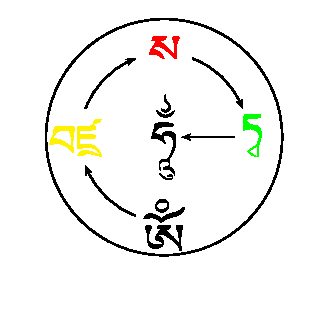
\includegraphics[bb=71 606 186 721]{heart}
\scaption{Roue du c{\oe}ur}
\end{figure}
\end{multicols}

\bigskip\bigskip

\titlesubsec{Dissolution}

\begin{tabbing}
\=\stib{'od zhu bdag snang dang 'dres ro gcig gyur\notsheg:}\\
\>\lit{�}---------------\=\lit{shu} \ \=\lit{dag-nang}
\=\lit{dang} \=\lit{dre} \quad \ \ \=\lit{ro}-----\=\lit{chig}
\=\lit{gyur}\\
\>\lex{(en) lumi�re} \>\lex{fond} \>\lex{perceptions}
\>\lex{avec} \>\lex{(se) m�le} \>\lex{saveur} \>\lex{unique}
\>\lex{devenir}\\
\>\trans{Il fond en lumi�re et se m�le � mes perceptions, en une
saveur unique.}
\end{tabbing}

%%-*-latex-*-

\begin{figure}[H]
\centering
\fbox{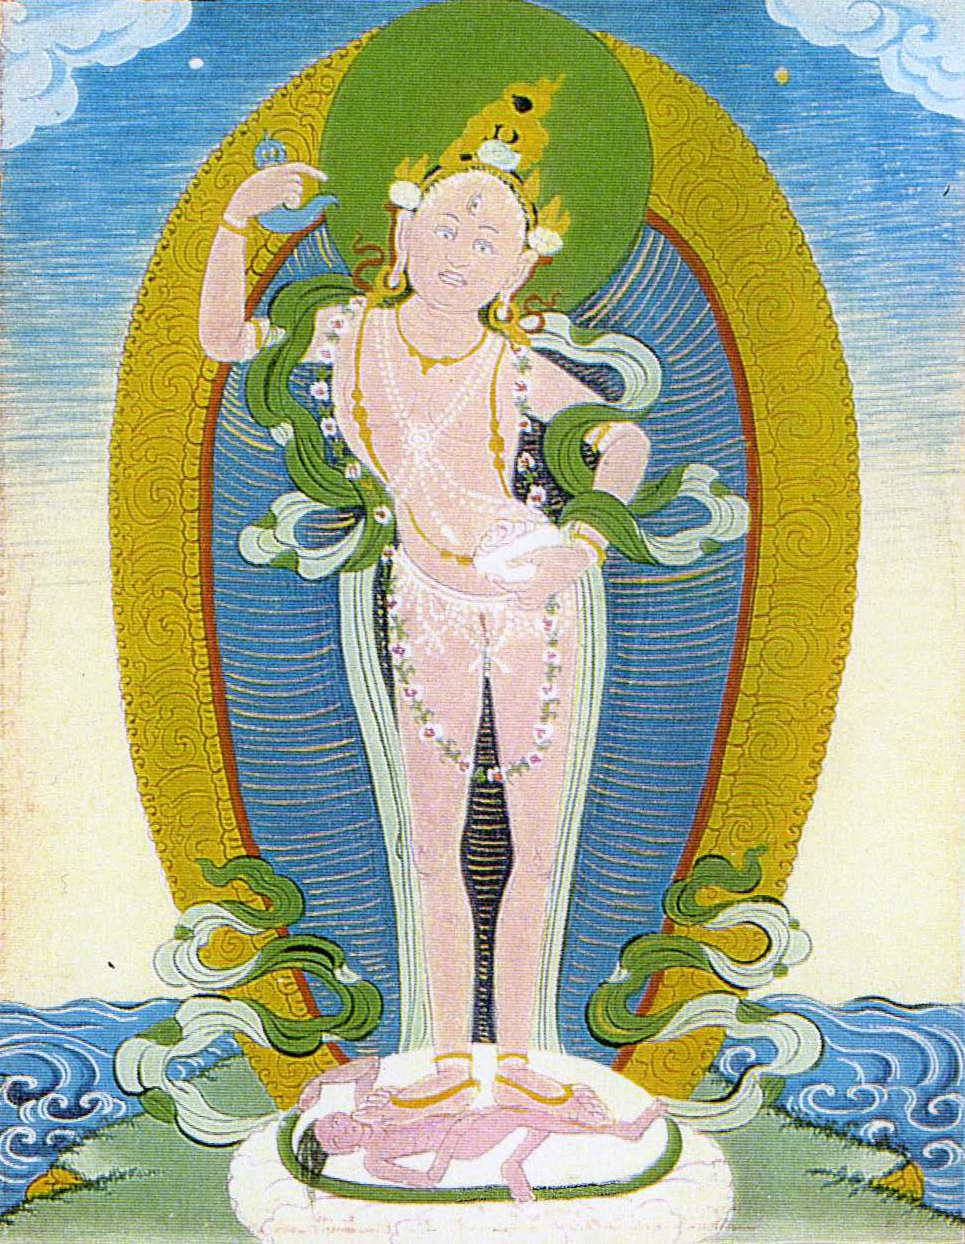
\includegraphics[scale=0.5]{vajrayogini-white.eps}}
\scaption{Vajrayogin\={\i} blanche (tib. N\={a}ro Khatch�ma)}
\end{figure}

\newpage

\titlesec{Union avec le ma�tre}
\addcontentsline{toc}{section}{\protect\numberline{}Union
  avec le ma�tre}

\bigskip\bigskip\bigskip

\titlesubsec{Cr�ation}

\begin{tabbing}
\=\stib{rang nyid rdo rje rnal 'byor mdun mkha' ru\notsheg:}\\
\>\lit{rang}-\lit{nyi} \=\lit{dorje} \lit{neljor}
\=\lit{d�n} \ \=\lit{kha} \=\lit{ru}\\
\>\lex{soi-m�me} \>\lex{Vajrayogin\a={\i}} \>\lex{devant}
\>\lex{ciel} \>\lex{dans}\\
\>\trans{Je suis Vajrayogin\a={\i}\sendnote{Vajrayogin\a={\i}
  est une \emph{\d{d}\a={a}kin\a={\i}} de sagesse (cf. note 3), qui
  poss�de plusieurs aspects. Celui repr�sent� ici est appel�
  N\={a}ro Khatch�ma en tib�tain, o� elle est blanche, portant
  seulement une tiare et des bijoux (symboles de la multiplicit� et
  de la brillance de la r�alit� manifeste). Elle pi�tine le cadavre de
  l'ego, l�ve le bras droit qui tient la lame courbe rituelle qui
  tranche les vues erron�es, et tient de l'autre main une calotte
  cr�nienne emplie d'ambroisie, signe qu'elle est au-del� du cycle de
  la naissance et de la mort.}
et dans le ciel devant moi}\\
\>\stib{rtsa ba'i bla ma pa\V{da}{ma}'i skur bzhengs gyur\notsheg:}\\
\>\lit{tsawa} \=\lit{lama} \=\lit{pem�} \qquad \=\lit{kur}-\=\lit{sheng}
\=\lit{gyur}\\
\>\lex{racine} \>\lex{ma�tre} \>\lex{N�-du-Lotus} \>\lex{corps}
\>\lex{appara�t} \>\lex{devenir}\\
\>\trans{se tient le ma�tre principal\sendnote{Le ma�tre principal est
  le ma�tre qui nous a transmis le texte pr�sent et autoris� les
  pratiques aff�rentes, qu'il a expliqu�es.} sous la forme de
  Guru Rinpoche.}\endnotemark[2]
\end{tabbing}

\newpage

\titlesubsec{Pri�re}

\begin{tabbing}
\=\stib{dus gsum sangs rgyas ma lus 'dus pa'i sku\notsheg:}\\
\>\lit{d�}-----\=\lit{sum} \=\lit{sangye} \=\lit{ma-l�} \qquad\
\=\lit{d�p�} \quad \=\lit{ku}\\
\>\lex{temps} \>\lex{trois} \>\lex{�veill�s} \>\lex{sans exception}
\>\lex{rassemble} \>\lex{incarnation}\\
\>\trans{Incarnation de tous les �veill�s du pass�, du pr�sent et du
futur,}\\
\>\stib{rtsa ba'i bla ma mchog la gsol ba 'debs\notsheg:}\\
\>\lit{tsaw�} \=\lit{lama} \=\lit{chog}---\=\lit{la}
\=\lit{s�lwa deb}\\
\>\lex{racine} \>\lex{ma�tre} \>\lex{excellent} \>\lex{�}
\>\lex{je prie}\\
\>\trans{excellent ma�tre principal, je vous prie!}\\
\>\stib{'di phyi bar do gsum du thugs rjes zungs\notsheg:}\\
\>\lit{di} \qquad \=\lit{chi} \=\lit{bardo} \quad
\=\lit{sum}-\=\lit{du} \=\lit{thugje} \ \=\lit{sung}\\
\>\lex{pr�sent} \>\lex{futur} \>\lex{tib. \emph{bardo}}
\>\lex{trois} \>\lex{en} \>\lex{compassion} \>\lex{tenez (moi)}\\
\>\trans{En cette vie, la prochaine et entre-deux,
soyez compatissant}\\
\>\stib{dus gsum rgyun chad med par byin gyis rlobs\notsheg:}\\
\>\lit{d�}-----\=\lit{sum} \=\lit{gy�n} \=\lit{cheme}-\=\lit{bra}
\=\lit{jin} \qquad \quad \ \=\lit{gyi} \=\lit{lob}\\
\>\lex{temps} \>\lex{trois} \>\lex{flot} \>\lex{continu} \>\lex{en}
\>\lex{b�n�dictions} \>\lex{accordez}\\
\>\trans{et que vos b�n�dictions se d�versent en flots continus!}
\end{tabbing}

\rep{� r�citer trois fois les mains jointes en pri�re.}

\bigskip\bigskip

\titlesubsec{Formule}

\begin{tabbing}
\=\stib{\om:} \ \stib{\V{a}{'}\notsheg:} \ \stib{\myhung\notsheg:}
\ \stib{badzra guru pa\V{da}{ma} si\V{di}{dh}\notsheg}
\ \stib{\myhung\notsheg:}\\
\>\lit{om} \quad \=\lit{ah} \quad \=\lit{hung}
\=\lit{benzer}
\ \=\lit{guru}--\=\lit{pema} \ \=\lit{siddhi}
\qquad\quad\ \=\lit{hung}\\
\>o\d{m}\endnotemark[12] \>\a={a}\d{h}\endnotemark[14]
\>h\a={u}\d{m}\endnotemark[4]
\>\sans{vajra} \>\sans{guru} \>\sans{padma} \>\sans{siddhi}
\>\sans{h\a={u}\d{m}}\\
\>\lex{(�veil en) Trois Corps}\sendnote{Les
  Trois Corps (\emph{trik\={a}ya}) sont trois aspects coessentiels �
  l'�veil, distingu�s uniquement dans un but didactique. Si la nature
  des Trois Corps est la m�me pour tous les �tres, chacun atteint
  l'�veil personnellement, c'est-�-dire actualise les Trois Corps.
  \begin{enumerate}
    \item Le premier corps est le �~corps cosmique~�
      (\emph{dharmak\={a}ya}), qui symbolise � la fois la dimension de
      vide d'existence intrins�que et la sagesse. On le compare, dans
      un but didactique, � une base indissoci�e d'un potentiel
      d'�mergence, ou � un germe d'�veil
      (\emph{tath\={a}gatagarbha}). On traduit ici aussi par �~r�alit�
      absolue~�.
    \item Le deuxi�me corps est le �~corps de fruition~�
      (\emph{sa\d{m}bhogak\={a}ya}), qui repr�sente l'�veil en
      mouvement pour le bien d'autrui, des reflets du
      \emph{dharmak\={a}ya} apparaissant par compassion. On le compare
      � la cause de l'�veil d'autrui. On traduit ici par �~r�alit�
      manifeste~� cette efflorescence.
    \item Le troisi�me corps est le
      \emph{nirm\={a}\d{n}ak\={a}ya}, le �~corps de manifestation~�,
      qui symbolise la forme que prend l'�veil pour aider les �tres,
      typiquement un corps illusoire ayant l'apparence salvifique
      idoine. On pourrait le comparer � un fruit m�r.
  \end{enumerate}
  Dans la perspective de la Grande Perfection (tib. Dzogchen,
  skt. Mah\={a}sa\.{n}dhi), les Trois Corps sont potentiellement
  contenus dans la base primordiale, leur �mergence compl�te et la
  reconnaissance de leur nature constituant la r�alisation de l'�veil
  complet. Le \emph{dharmak\={a}ya} correspond alors � l'essence vide,
  le \emph{sa\d{m}bhogak\={a}ya} � la nature lumineuse de l'�tre et le
  \emph{nirm\={a}\d{n}ak\={a}ya} � l'�nergie compatissante au
  service d'autrui.}  \>\>\>\lex{infrangible} \>\lex{ma�tre}
\>\lex{lotus} \>\lex{accomplissements}
\>\lex{(scellement)}\\ \>\trans{Les purifications (des roues) du
  corps, de la parole et de l'esprit}\\ \>\trans{m�nent aux
  acccomplissements de l'infrangible Ma�tre du Lotus.}\\ \>\trans{Les
  accomplissements du Ma�tre du Lotus sont l'�veil
  infrangible}\\ \>\trans{et complet.}
\end{tabbing}

\rep{� r�citer autant de fois que possible.}

\newpage

\titlesubsec{Scellement}

\begin{tabbing}
\=\stib{sku gsung thugs kyi dbang byin yongs rdzogs thob\notsheg:}\\
\>\lit{ku} \ \ \=\lit{sung} \=\lit{thug} \=\lit{kyi}
\=\lit{wang}---\=\lit{jin} \qquad\qquad \=\lit{yong}---\=\lit{dzog}
\ \=\lit{thob}\\
\>\lex{corps} \>\lex{parole} \>\lex{esprit} \>\lex{de}
\>\lex{initiations} \>\lex{b�n�dictions} \>\lex{complet} \>\lex{parfait}
\>\lex{obtenir}\\
\>\trans{Initiations et b�n�dictions\sendnote{L'initiation
  (\emph{abhi\d{s}eka}) est, litt�ralement, une ablution rituelle
  qui rend manifeste une qualit� de l'�veil. Elle est requise pour
  quiconque souhaite s'engager dans la pratique d'un enseignement du
  \emph{tantra} (skt.) et elle est conf�r�e par un ma�tre ayant r�alis�
  lui-m�me les fruits de la pratique en question. Ici, ce yoga de
  l'union avec le ma�tre correspond � une initiation rituelle conf�r�e
  par Guru Rinpoche et le fruit de la pratique, c'est-�-dire la
  reconnaissance de la nature de l'esprit du ma�tre en soi-m�me, est
  la b�n�diction (\emph{adhi\d{s}\d{t}h\={a}na}), c'est-�-dire
  l'�closion des qualit�s spirituelles.} des corps, parole et esprit
  sont int�gralement }\\
\>\trans{re�ues.}\\
\>\stib{badzra gu ru \V{ka}{'} ya \V{la}{\V{ba}{'}}ka tsi\V{ta}{ta}
  si\V{di}{dh}   \myhung\notsheg:} \quad \textsf{\large[formule]}\\
\>\lit{benzra} \=\lit{guru} \=\lit{kaya} \=\lit{waka} \=\lit{tsitta}
\=\lit{siddhi} \qquad\qquad \=\lit{hung}\\
\>\sans{vajra} \>\sans{guru} \>\sans{k\a={a}ya} \>\sans{v\a={a}k}
\>\sans{citta} \>\sans{siddhi} \>\sans{h\a={u}\d{m}}\\
\>\lex{infrangible} \>\lex{ma�tre} \>\lex{corps} \>\lex{parole}
\>\lex{esprit} \>\lex{accomplissements} \>\lex{(scellement)}\\
\>\trans{Le corps, la parole et l'esprit du ma�tre sont immuablement
r�alis�s}\\
\>\trans{(en soi).}
\end{tabbing}

\bigskip\bigskip

\titlesubsec{Dissolution}

\begin{tabbing}
\=\stib{bla ma 'od zhu rang thim dbyer med ngang\notsheg:}\\
\>\lit{lama} \=\lit{�}--------\=\lit{shu} \ \ \=\lit{rang}
\=\lit{thim} \=\lit{yerme} \ \ \=\lit{ngang}\\
\>\lex{ma�tre} \>\lex{lumi�re} \>\lex{dissout} \>\lex{soi}
\>\lex{dissout} \>\lex{ins�parable} \>\lex{(je) demeure}\\
\>\trans{Le ma�tre se dissout en une lumi�re qui se fond en moi,}\\
\>\trans{et ainsi je demeure,}\\
\>\stib{rig stong don gyi bla ma'i rang zhal balta\notsheg:}\\
\>\lit{rig}---------\=\lit{tong} \=\lit{d�n}-\lit{gyi} \=\lit{lam�}
\=\lit{rang}-\=\lit{shel} \=\lit{ta}\\
\>\lex{conscience} \>\lex{vide} \>\lex{sens vrai} \>\lex{ma�tre}
\>\lex{propre} \>\lex{visage} \>\lex{(je) contemple}\\
\>\trans{contemplant la conscience vide, vrai visage du ma�tre.}
\end{tabbing}

%%-*-latex-*-

\vspace*{\stretch{1}}
\begin{figure}[H]
\centering
\fbox{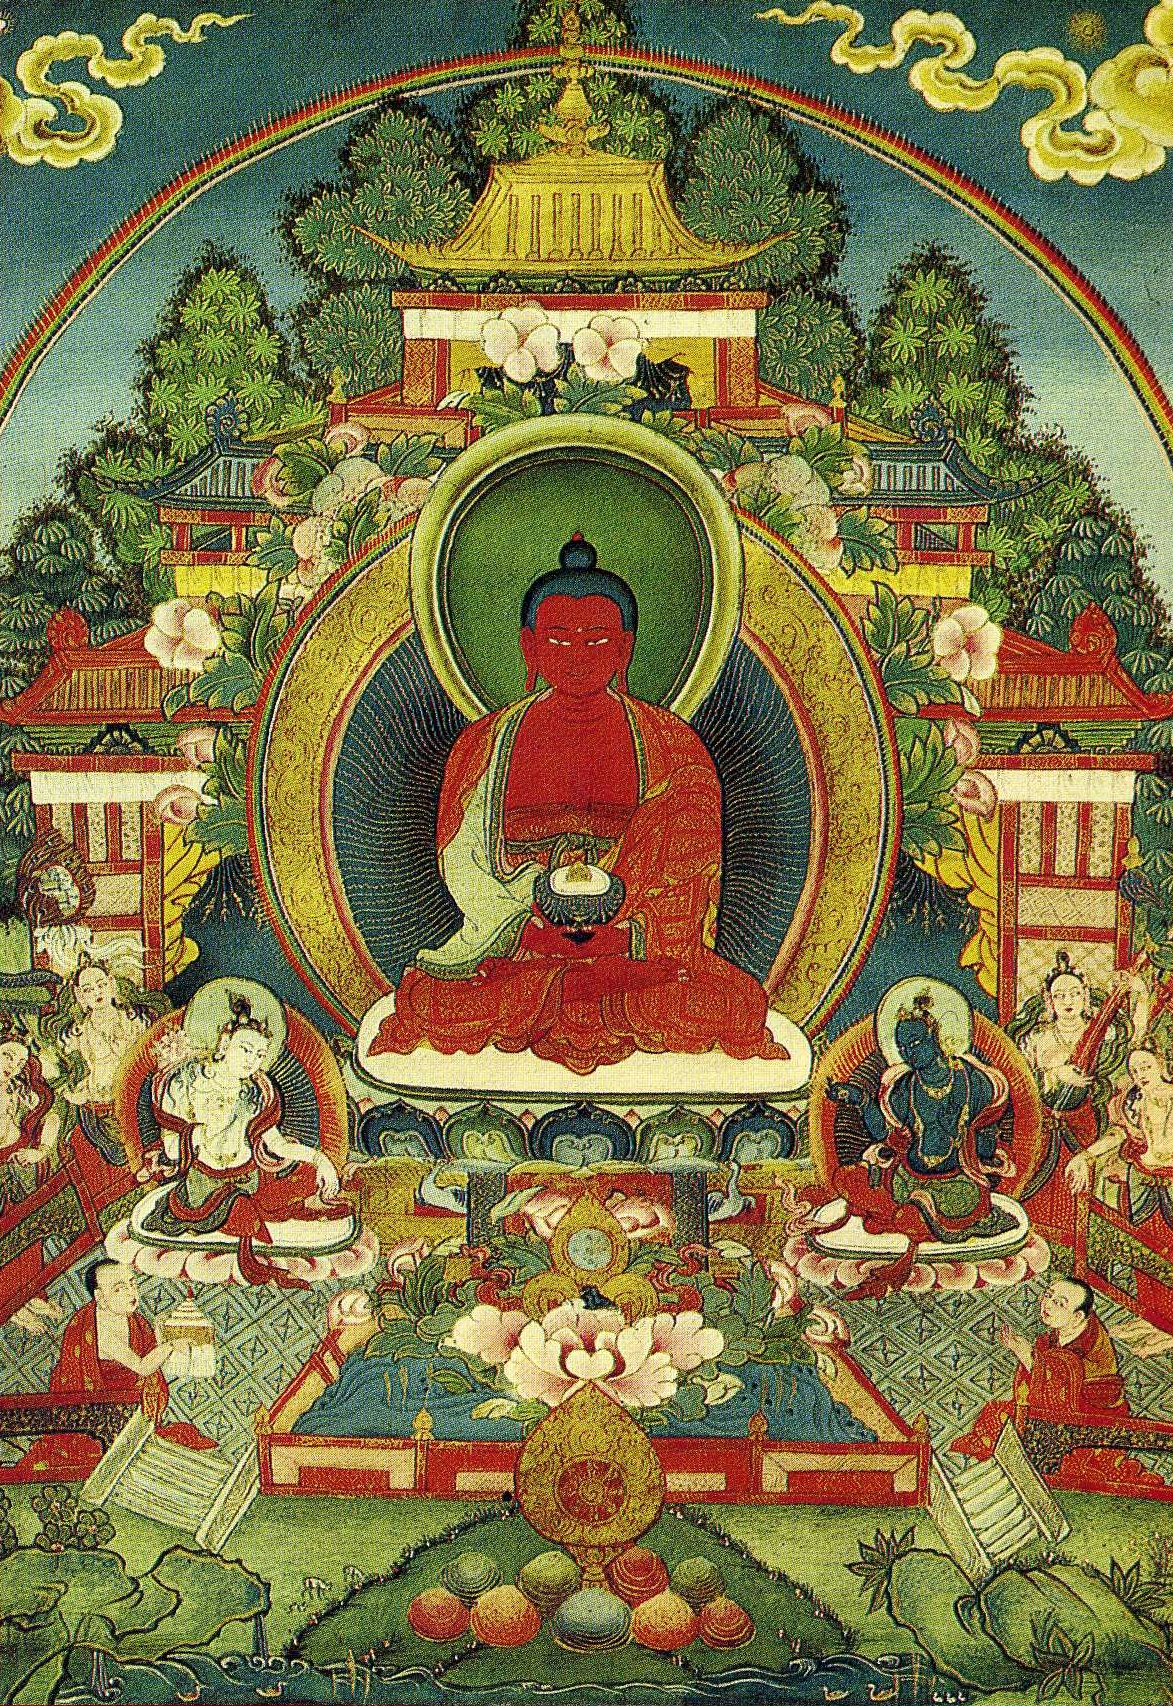
\includegraphics[scale=0.4]{amitabha.eps}}
\scaption{Le Vainqueur Amit\a={a}bha}
\end{figure}
\vspace*{\stretch{1}}

\newpage

\titlesec{Transfert de la conscience}
\addcontentsline{toc}{section}{\protect\numberline{}Transfert de la conscience}

\bigskip\bigskip

\begin{tabbing}
\=\stib{mgon po 'od dpag med la gsol ba 'debs\notsheg:}\\
\>\lit{g�npo} \quad \=\lit{�}---------\=\lit{pagme} \=\lit{la}
\=\lit{s�lwa} \lit{deb}\\
\>\lex{protecteur} \>\lex{lumi�re} \>\lex{infinie} \>\lex{�}
\>\lex{je prie}\\
\>\trans{� Protecteur Amit\a={a}bha,\sendnote{Le Vainqueur (ou
  Protecteur) Amith\={a}bha est le repr�sentant de la famille du lotus
  (cf. note~5). Il sert ici de support � une pratique de
transfert de la conscience du mourant dans la Terre Pure de l'Ouest
(Sukh\={a}vat\={\i}), sur laquelle il r�gne. Il est
repr�sent� assis en lotus sur un tr�ne de lotus; ses mains font le
sceau (\emph{mudr\={a}}) du recueillement m�ditatif, et tiennent
un bol � aum�nes empli d'ambroisie. Il est flanqu�
de deux acolytes (\emph{bodhisattva}): � sa droite,
Avalokite\'{s}vara, blanc et tenant une fleur de lotus par la tige; �
sa gauche, Mah\={a}sth\={a}mapr\={a}pta (identifi� � Vajrap\={a}\d{n}i
d'apparence paisible dans le Vajray\={a}na), bleu et tenant un
\emph{vajra}. Ces deux assistants repr�sentent respectivement la
compassion en tant que sagesse et la compassion en tant qu'�nergie
salvifique. La rutilance illimit�e et isotrope d'Amit\={a}bha
caract�rise la compassion sans bornes et impartiale, pr�sente
potentiellement en chaque �tre (cf. l'\emph{Appel du ma�tre qui est au
  loin}, page~\pageref{compassion}) pour le b�n�fice d'autrui. Le
transfert de la conscience n'est ici qu'effleur� et n'est r�ellement mis
en pratique qu'apr�s que les pr�liminaires extraordinaires ont �t�
accomplis.} je vous prie}\\
\>\stib{zab lam 'pho ba 'byongs bar byin gyis rlobs\notsheg:}\\
\>\lit{sab}--------\=\lit{lam} \=\lit{phowa} \quad \=\lit{jong}-\lit{bra}
\=\lit{jin} \qquad \quad \=\lit{gyi} \=\lit{lob}\\
\>\lex{profonde} \>\lex{voie} \>\lex{tib. \emph{phowa}}
\>\lex{parfait dans} \>\lex{b�n�diction} \>\lex{par}
\>\lex{accordez}\\
\>\trans{de me b�nir afin que j'accomplisse la voie profonde du
transfert}\\
\>\trans{de conscience!}
\end{tabbing}

\rep{� r�citer trois fois.}

\newpage

\vspace*{\stretch{1}}
\begin{figure}[H]
\centering
\fbox{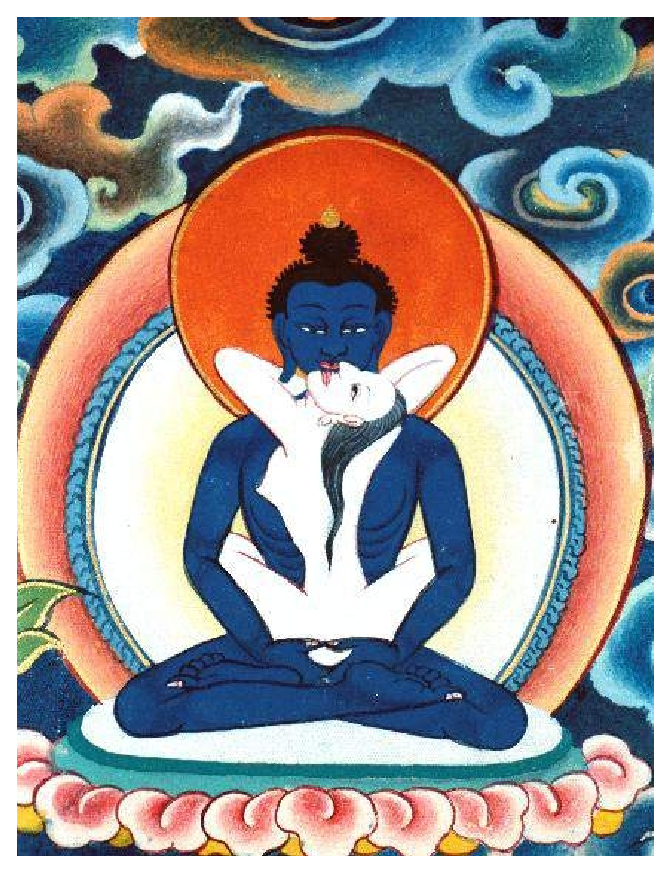
\includegraphics[scale=0.7]{samantabhadra.eps}}
\scaption{L'�veill� primordial Samantabhadra}
\end{figure}
\vspace*{\stretch{1}}

%%-*-latex-*-

\titlesec{D�dicace des m�rites}
\addcontentsline{toc}{section}{\protect\numberline{}D�dicace des m�rites}

\bigskip\bigskip

\begin{tabbing}
\=\stib{da ni lus dang longs spyod dge rtsar bcas\notsheg:}\\
\>\lit{dani} \qquad \=\lit{l�} \quad \=\lit{dang}
\=\lit{long}-\lit{ch�} \=\lit{ge} \quad \=\lit{tsar} \=\lit{che}\\
\>\lex{maintenant} \>\lex{corps} \>\lex{et} \>\lex{possessions}
\>\lex{vertu} \>\lex{racine} \>\lex{ensemble}\\
\>\trans{Maintenant, mon corps, mes biens et la racine de mes vertus,}\\
\>\stib{ma gyur 'gro la phangs pa med par btang\notsheg:}\\
\=\lit{ma}--\=\lit{gy�r} \quad \=\lit{dro}--\=\lit{la}
\=\lit{phang}-\lit{pa} \=\lit{me}-\lit{pra} \=\lit{tang}\\
\>\lex{m�re} \>\lex{ayant �t�} \>\lex{�tres} \>\lex{�}
\>\lex{attachement} \>\lex{sans} \>\lex{je donne}\\
\>\trans{je les donne sans retenue � tous les �tres, mes anciennes
m�res;}\\
\>\stib{'gro don rlabs chen gegs med 'grub par shog\notsheg:}\\
\=\lit{dro}--\=\lit{d�n} \quad \=\lit{lab} \quad \=\lit{chen}
\=\lit{geg}--\lit{me} \quad \ \=\lit{drub}--\lit{pra} \=\lit{shog}
\textbf{\large [bis]}\\
\>\lex{�tres} \>\lex{b�n�fice} \>\lex{grandes} \>\lex{vagues}
\>\lex{sans obstacles} \>\lex{s'accomplir} \>\lex{puisse}\\
\>\trans{que le bien de tous les �tres s'accomplisse en grandes vagues}\\
\>\trans{sans obstacles!}
\end{tabbing}


\cleardoublepage
%%-*-latex-*-

\addcontentsline{toc}{chapter}{\protect\numberline{}Notes}

\bigskip\bigskip

\theendnotes

\listoffigures
\addcontentsline{toc}{chapter}{\protect\numberline{}Table des figures}
%%-*-latex-*-

\pagestyle{empty}
\cleardoublepage
\
\cleardoublepage
\ 
\clearpage
\ 

\vfill

\begin{center}
\normalsize
\textbf{Shedup K�nsang Ch�ling}\\
2, Rue de la Basse Cour\\
Place de la Mairie\\
F-02410 \quad Septvaux\\
France\\
\bigskip
+33 (0)3.23.52.09.93\\
\url{skc02@free.fr}\\
\url{http://www.shedup-kunsang-choling.com/}
\end{center}



\end{document}
